% To compile:
% pdflatex report.tex

% ==============================================================
% Latex packages and settings
% ==============================================================
\documentclass[11pt]{article}

% Language setting:
% Replace `english' with e.g. `spanish' to change the document language
\usepackage[english]{babel}                             % Set document language (hyphenation, date formats, etc.)

% Set caption formatting:
\usepackage{caption}                                    % Control the appearance of figure and table captions
\captionsetup[table]{labelfont=bf, font=small}          % Make table labels bold and use a small font for table captions
\captionsetup[figure]{labelfont=bf, font=small}         % Make figure labels bold and use a small font for figure captions

\usepackage{subcaption}                                 % Allow subFigures_compressed/subtables with individual sub-captions

% Set page size and margins:
% Replace `letterpaper' with `a4paper' for UK/EU standard size
\usepackage[a4paper,top=2cm,bottom=2cm,left=2.5cm,right=2.5cm,marginparwidth=1.75cm]{geometry} % Configure paper size and margins

% Useful packages
\usepackage{amsmath}                                    % Enhanced math environments and symbols
\usepackage{amssymb}                                    % Additional math symbols
\usepackage{graphicx}                                   % Include and scale external graphics (e.g. .pdf, .png)
\usepackage[colorlinks=true,                            % Use colored links instead of boxed links
            allcolors=blue,                             % Use blue for all link types (cite, ref, url)
            bookmarksnumbered=true,                     % Number the PDF bookmarks according to section numbers
            bookmarksopen=true,                         % Open the bookmark tree when the PDF is opened
            bookmarksopenlevel=10]{hyperref}            % Control depth to which bookmarks are expanded
\usepackage{listings}                                   % Typeset source code with syntax highlighting

\usepackage{authblk}                                    % Manage authors and affiliations in a structured way
% Make only the author and/or affiliation smaller
% \renewcommand\Authfont{\small}                        % Set the Author font size (e.g. small or footnotesize)
\renewcommand\Affilfont{\small}                         % Set the affiliation font size (e.g. small or footnotesize)
\renewcommand\Authand{}        % <-- add this

\usepackage{comment}                                    % Define large comment environments to exclude blocks from output
\usepackage{enumitem}                                   % Customize list environments (itemize, enumerate, etc.)
\usepackage{lineno}                                     % Add optional line numbers to the document
% \usepackage[backend=biber, style=numeric-comp, citestyle=numeric-comp, sorting=none]{biblatex} % Modern bibliography management with biber backend
\usepackage[backend=biber, sorting=none, style=numeric, citestyle=numeric]{biblatex} % Modern bibliography management with biber backend
\addbibresource{../references.bib}                     % Load bibliography entries for citations and references
% Make bibliography font smaller
\renewcommand*{\bibfont}{\footnotesize}                 % Reduce font size in the bibliography
\usepackage{multirow}                                   % Enable table cells that span multiple rows
\usepackage{rotating}                                   % Rotate figures, tables, or text (e.g. sideways tables)
\usepackage{pdfpages}                                   % Include external PDF pages in the document
\usepackage{csquotes}                                   % Context-sensitive quotation marks, recommended with biblatex
\usepackage[table]{xcolor}                              % Color support, including coloring table rows/columns
\usepackage{array, makecell, colortbl}                  % Extra tools for tables: new column types, multi-line cells, colored cells
\renewcommand{\arraystretch}{1.5}                       % Increase row height in tables by a factor of 1.5
% \setlength{\parskip}{1\baselineskip}                    % Adds a full line space between paragraphs
\setlength{\parindent}{0pt}                             % Optional: removes paragraph indentation

\usepackage{sidecap}

% ==============================================================
% Document title and author
% ==============================================================
\title{\textbf{Numerov Method for Bound States in the One-Dimensional Schr\"odinger Equation}}
\author{Alon Sportes (ID: 204498745)}
\date{}

% ==============================================================
% Document content
% ==============================================================
\begin{document}
    \maketitle

    \vfill

    \phantomsection
    \begingroup
        \setlength{\parskip}{0pt}
        \addcontentsline{toc}{section}{Table of Contents}
        \tableofcontents
    \endgroup
    \vfill

    % Start citation tracking here
    \begin{refsection}

    \newpage

    % ==============================================================
    % Introduction
    % ==============================================================
    \section{Introduction}
        This project studies the one-dimensional time-independent Schr\"odinger equation using the Numerov method combined with parity-aware shooting procedures. The goals are to validate the method on systems with known analytic solutions, demonstrate numerical convergence and accuracy, and then apply it to more interesting bound-state potentials such as a double well and a finite square well. Extensions to scattering problems are also explored as a secondary component. \\

        This problem is a boundary-value eigenvalue problem rather than a standard initial-value problem: only special energies produce wavefunctions satisfying the required boundary behavior. The Numerov method is well suited to this task because the time-independent Schr\"odinger equation has the second-order form $\psi''=q(x)\psi$, with no first-derivative term. The project therefore focuses not only on obtaining eigenvalues, but also on checking that the numerical results are physically meaningful through analytic benchmarks, convergence tests, parity and node structure, and probability conservation in the scattering extension. \\
        
        The full code was written in Python and is available in \href{https://github.com/alons126/Numerov-bound-states}{this repository}. The implementation is modular, with separate components for the Numerov integrator, shooting method, root finding, analysis utilities, and an automated validation suite. This structure allows for independent validation of each numerical component and makes the overall workflow easier to understand.

    % ==============================================================
    % Computational approach
    % ==============================================================
    \section{Computational approach}
        \subsection{The Schr\"odinger equation and Numerov method}
            In dimensionless units, the Schr\"odinger equation is written as:
            \begin{equation}
            \psi''(x) = 2\,[V(x)-E]\psi(x)
            \end{equation}
            The wavefunction is integrated with the Numerov scheme on a uniform grid. For symmetric potentials, even and odd states are treated separately using parity conditions at $x=0$. Eigenvalues are found by scanning for sign changes in a scalar mismatch function and then refining the resulting brackets with robust root finding; in the outward Numerov solver this is bisection followed by a few safeguarded secant-style polishing steps, while the inward-decay and RK4 solvers use straight bisection. The correctness of the numerical approach is verified through comparison with analytical solutions where available, through systematic convergence studies, and through direct automated tests of the implementation. \\

            The overall numerical workflow is implemented in a modular way in the accompanying Python code. The core components include a Numerov integrator for propagating the wavefunction, a shooting module that enforces parity-based boundary conditions and constructs the mismatch function, and analysis utilities for convergence studies and parameter sweeps. This separation of concerns allows each numerical component to be validated independently and makes the implementation easier to interpret \cite{Pang_2006}.

        \subsection{Shooting and root finding}
            The boundary-value eigenproblem is reformulated as a root-finding problem for a mismatch function $M(E)$. For a given trial energy $E$, the Schr\"odinger equation is integrated and a boundary mismatch is evaluated. The code uses two related formulations. For the infinite square well, finite square well, and quartic double well, the half-domain problem is shot outward from $x=0$ with parity-consistent startup values and the raw mismatch is the outer boundary value $M(E)=\psi_E(x_{\max})$. For the harmonic oscillator and the RK4 comparison, the code instead shoots inward from $x_{\max}$ through the decaying tail and enforces parity at the origin:
            \begin{align}
            \text{even states:}\quad M(E) = \psi'_E(0),\,\,\,\,\,\,\,\,\,\,\text{odd states:}\quad M(E) = \psi_E(0)
            \end{align}
            Eigenvalues correspond to the roots of $M(E)=0$, which are located by bracketing sign changes and then refined numerically. To make the procedure transparent, the report now uses two complementary diagnostics: a global raw-mismatch scan over the full energy interval, where only the final root estimates are marked, and per-root zoom plots that restrict the horizontal axis to one initial bracket and show the full bisection history. Zero crossings identify the allowed energies. \\

            In the implementation, the inward even-state mismatch uses a fourth-order backward finite-difference stencil to approximate $\psi'(0)$ from the last few points of the inward integration grid. This is important because a lower-order boundary derivative would spoil the fourth-order behavior otherwise expected from the Numerov recurrence in the harmonic-oscillator study.

    % ==============================================================
    % Results
    % ==============================================================
    \section{Results}
        Each potential is used to validate, test, or demonstrate different aspects of the numerical method, ranging from analytic benchmarks to nontrivial quantum behavior.

        \subsection{Infinite square well}
            The infinite square well serves as a benchmark problem with known analytic spectrum:
            \begin{equation}
            E_n = \frac{(n+1)^2\pi^2}{8a^2}
            \end{equation}
            The potential is:
            \begin{equation}
            V(x)=\begin{cases}
            0 & ,|x|\le a\\
            \infty & ,|x|>a
            \end{cases}
            \qquad \text{(implemented numerically with a large finite }V_0\text{)}
            \end{equation}
            In the production calculation, the well half-width is $a=1$, the outward-shooting half-domain uses $x_{\max}=a=1$, the Numerov grid uses $n_{\text{grid}}=2500$ points, and the numerical wall height is set to $V_0=10^6$. The grid-convergence study for this case uses $n_{\text{grid}}\in\{50,80,120,180\}$ at fixed $x_{\max}=1$. \\

            The numerical eigenvalues agree with the analytic values to essentially machine precision, as shown in Fig.~\ref{fig:infwell_energies}. In the saved run the first four relative errors are $4.9\times10^{-11}$, $1.3\times10^{-10}$, $2.6\times10^{-11}$, and $7.0\times10^{-12}$. This is exactly the behavior expected for a benchmark problem of this type: the energies follow the analytic law $E_n \propto (n+1)^2$, and the numerical points are visually indistinguishable from the exact curve on the scale of the plot. \\

            The probability densities for the first four states (Fig.~\ref{fig:infwell_densities}) also have the expected structure. The ground-state density is maximal at the center, while the excited states show the correct sequence of interior nodes inherited from the alternating even/odd parity eigenfunctions. All densities vanish at $x=\pm a$, consistent with the hard-wall boundary condition. \\

            The shooting method is validated by plotting the boundary mismatch functions for both even and odd sectors (Fig.~\ref{fig:infwell_shooting}). The even-sector scan has zero crossings near $E\approx1.234$ and $E\approx11.103$, while the odd-sector scan crosses zero near $E\approx4.935$ and $E\approx19.739$. These are precisely the first four physical eigenvalues, so the parity separation and bracketing logic are behaving as intended rather than picking spurious roots. \\

            The convergence of the energy error as a function of grid spacing $h$ (Fig.~\ref{fig:infwell_convergence}) is also as expected for Numerov. The fitted exponents from the saved convergence study are $p=3.94$, $4.00$, $3.98$, and $4.00$ for the first four states, which is strong evidence that the recurrence, startup values, and boundary treatment are all consistent with fourth-order accuracy. The higher states sit at larger absolute error for a fixed grid, which is also expected because their shorter wavelengths are harder to resolve. \\

            Finally, the wavefunctions for the first four states are plotted together with their corresponding energies and the confining potential (Fig.~\ref{fig:infwell_states}). The alternating parity, increasing node count, and quadratic growth of the energy levels all match the analytic infinite-well picture. \\

            \begin{figure}[p]
                \centering
                
                \begin{minipage}[t]{0.48\textwidth}
                    \centering
                    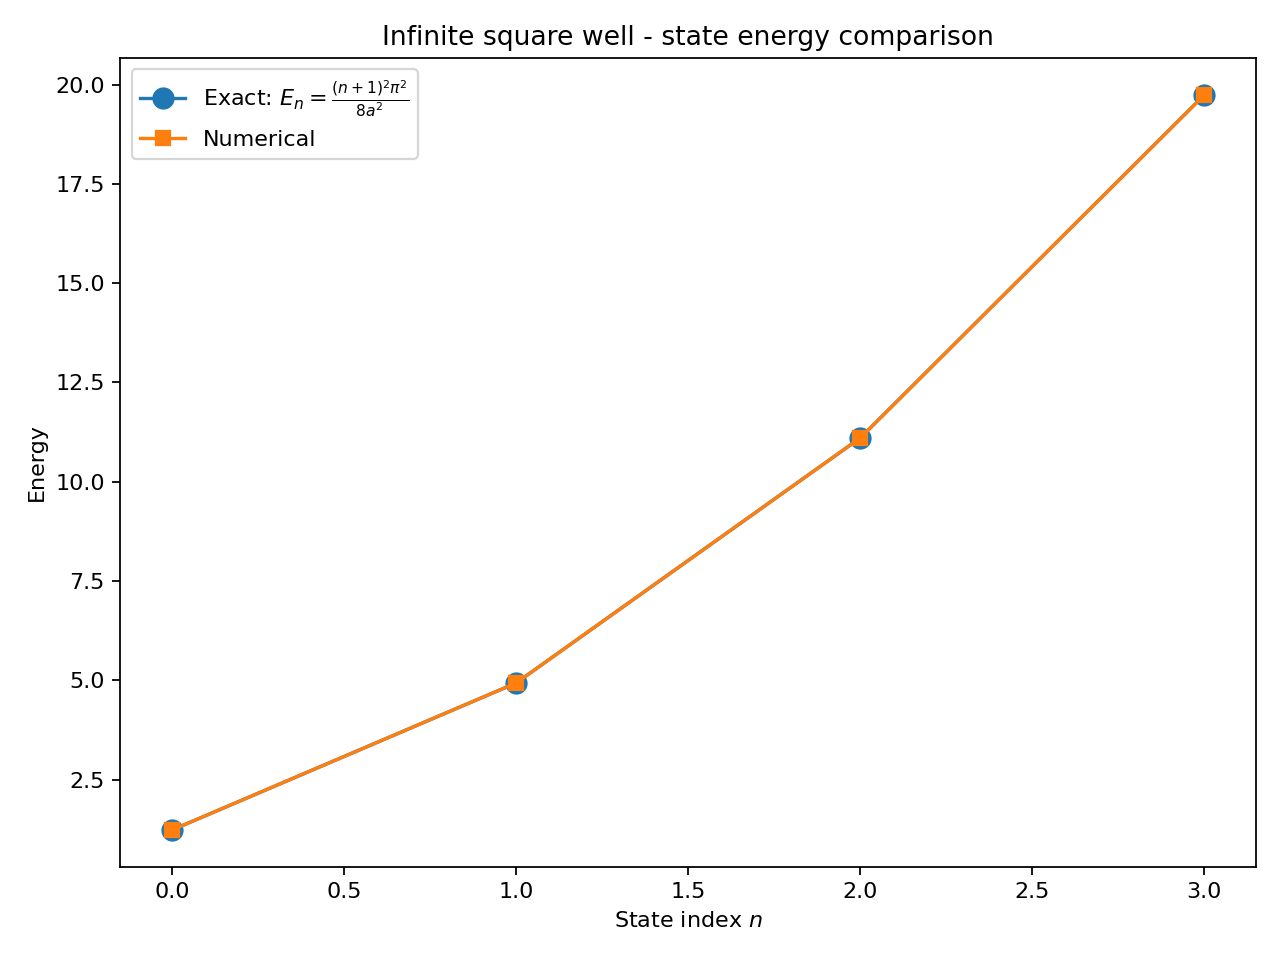
\includegraphics[width=\textwidth]{../../results/1_infinite_square_well_Numerov/1_infinite_square_well_Numerov_state_energy_comparison.png}
                    \captionof{figure}{Comparison between numerical and exact energy eigenvalues for the infinite square well. The agreement is excellent for the first four states.}
                    \label{fig:infwell_energies}
                \end{minipage}
                \hfill
                \begin{minipage}[t]{0.48\textwidth}
                    \centering
                    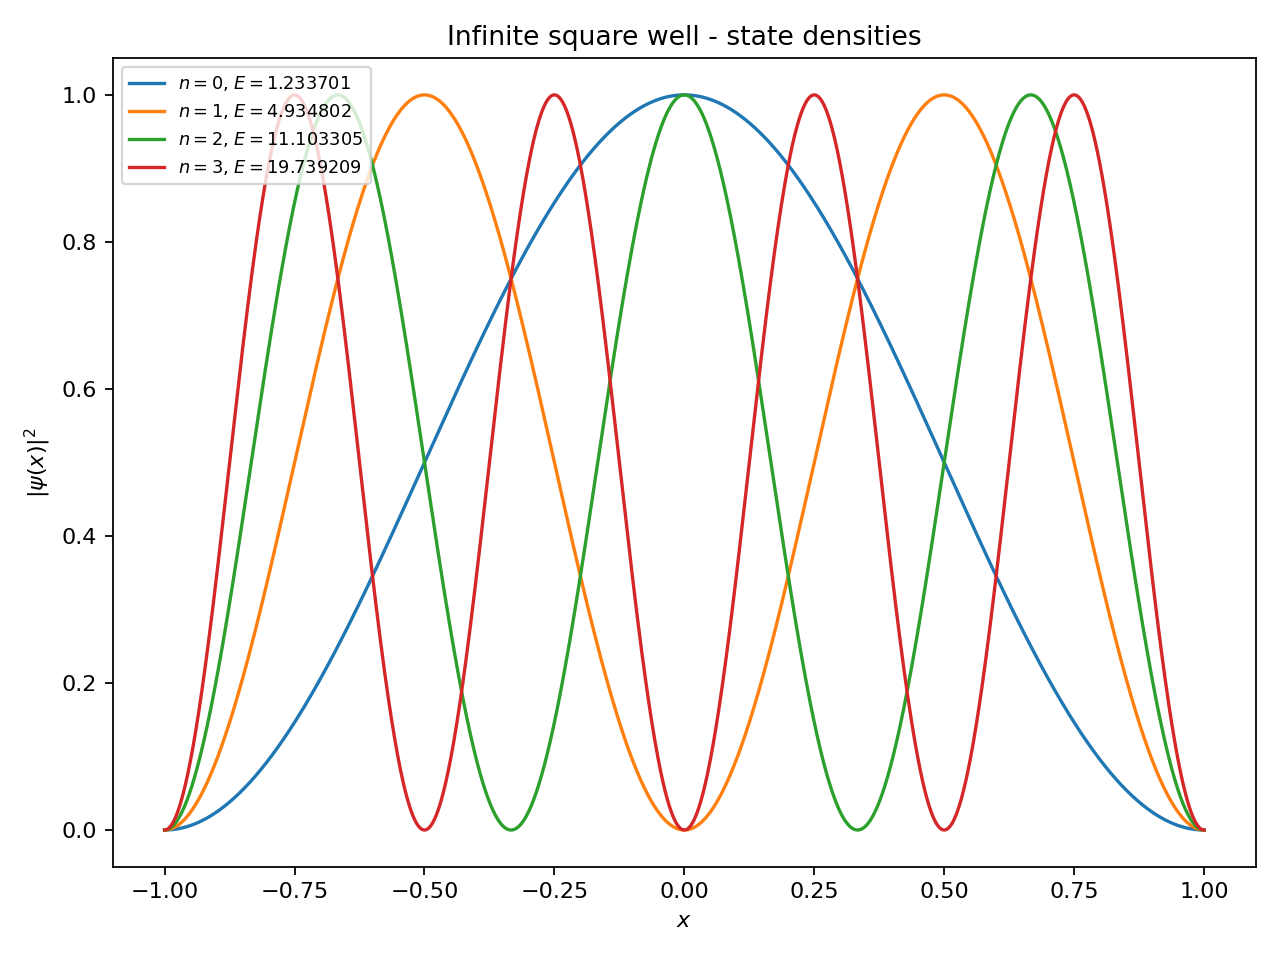
\includegraphics[width=\textwidth]{../../results/1_infinite_square_well_Numerov/1_infinite_square_well_Numerov_state_densities.png}
                    \captionof{figure}{Probability densities $|\psi(x)|^2$ for the first four eigenstates of the infinite square well. The correct number of nodes and boundary behavior are clearly reproduced.}
                    \label{fig:infwell_densities}
                \end{minipage}

                \vspace{1em}

                \begin{minipage}[t]{\textwidth}
                    \centering
                    \begin{subfigure}[t]{0.485\textwidth}
                        \centering
                        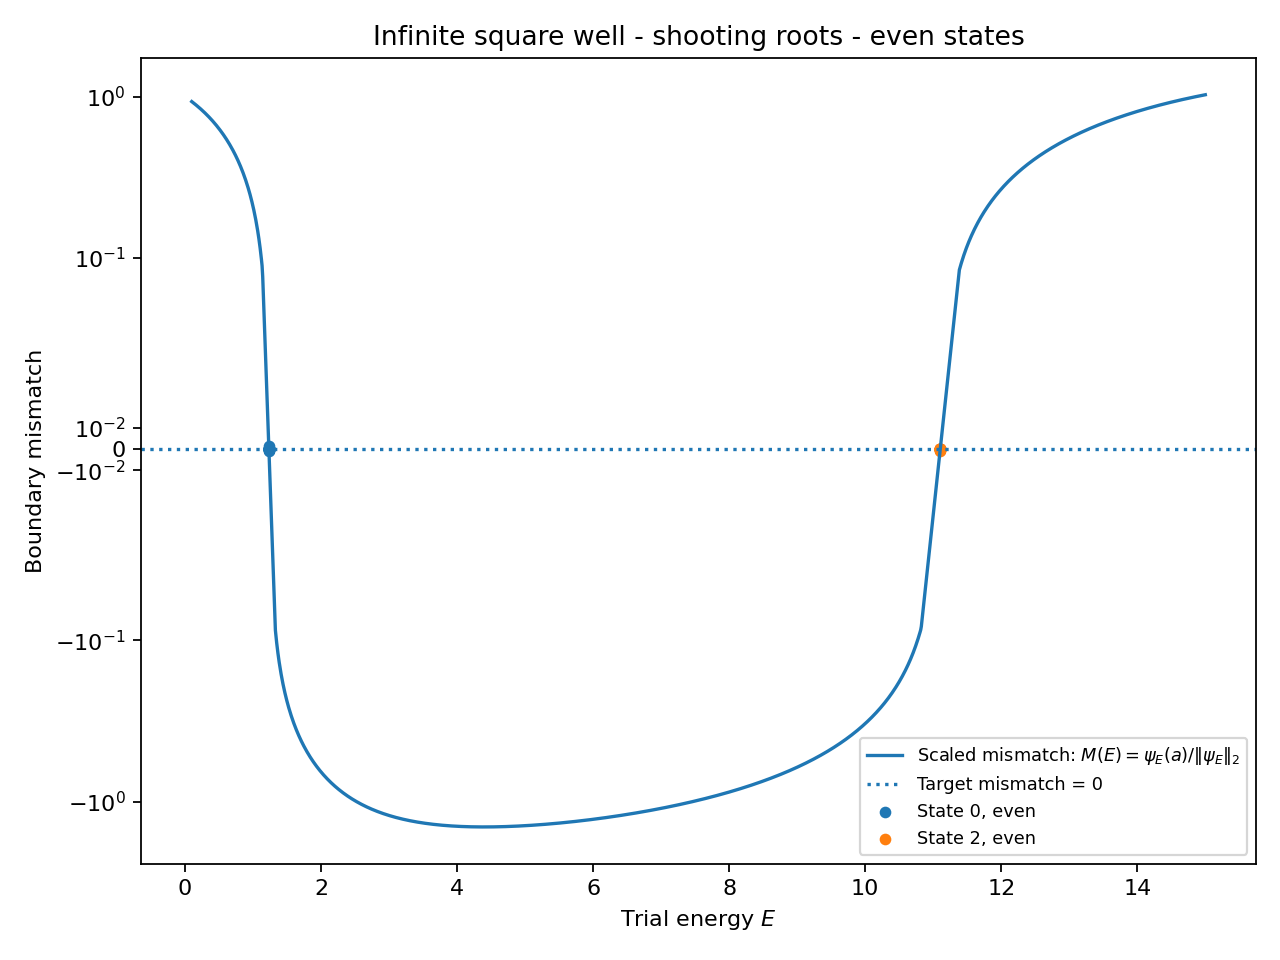
\includegraphics[height=5cm]{../../results/1_infinite_square_well_Numerov/1_infinite_square_well_Numerov_root_finding_even.png}
                        \caption{}
                    \end{subfigure}
                    \hfill
                    \begin{subfigure}[t]{0.485\textwidth}
                        \centering
                        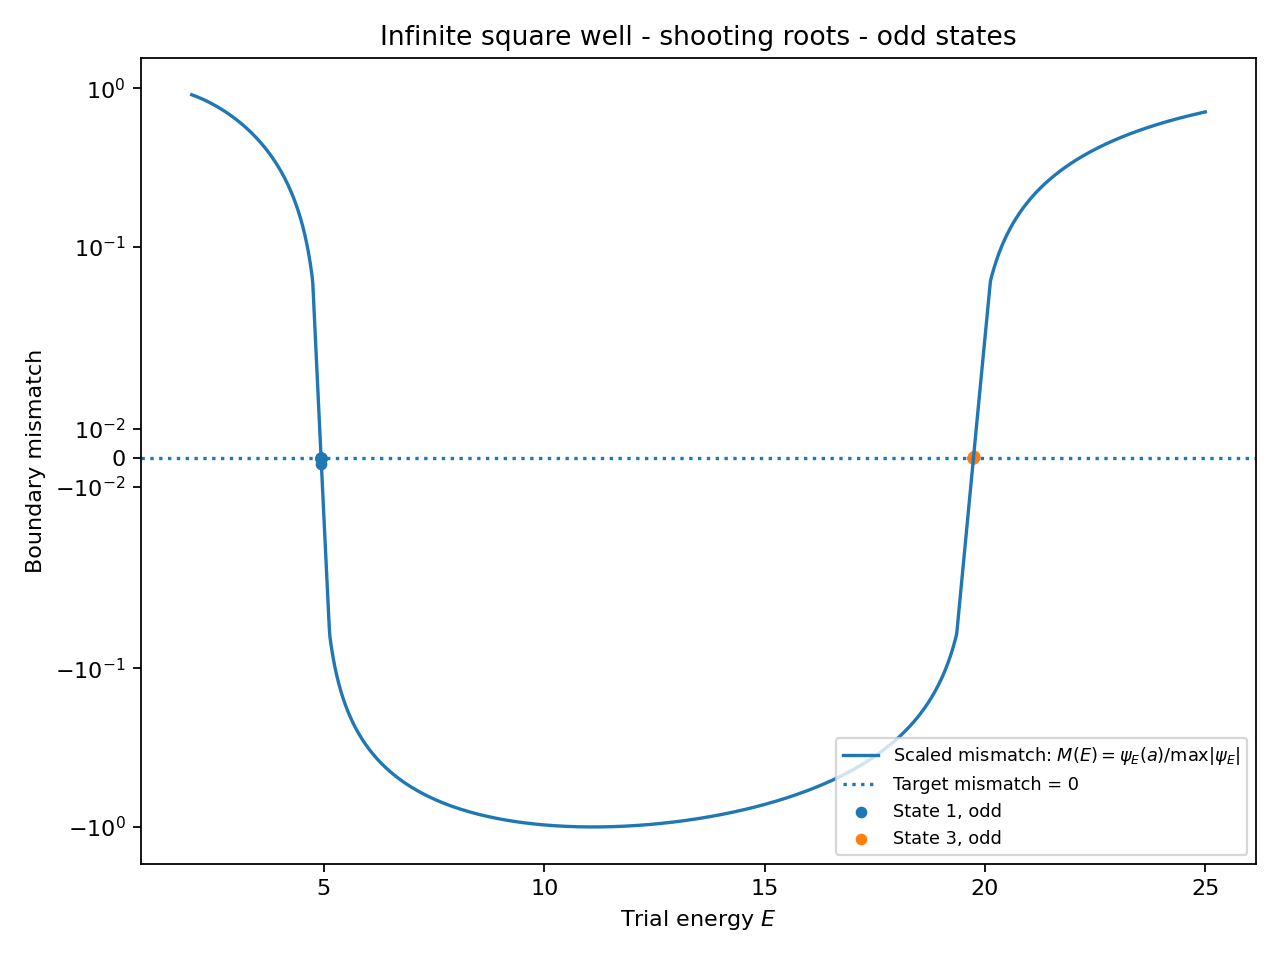
\includegraphics[height=5cm]{../../results/1_infinite_square_well_Numerov/1_infinite_square_well_Numerov_root_finding_odd.png}
                        \caption{}
                    \end{subfigure}

                    \captionof{figure}{Raw boundary mismatch functions for even (a) and odd (b) states. The zero crossings correspond to the physical eigenvalues found by the shooting method.}
                    \label{fig:infwell_shooting}
                \end{minipage}

                \vspace{1em}

                \begin{minipage}[t]{\textwidth}
                    \centering
                    \begin{subfigure}[t]{0.485\textwidth}
                        \centering
                        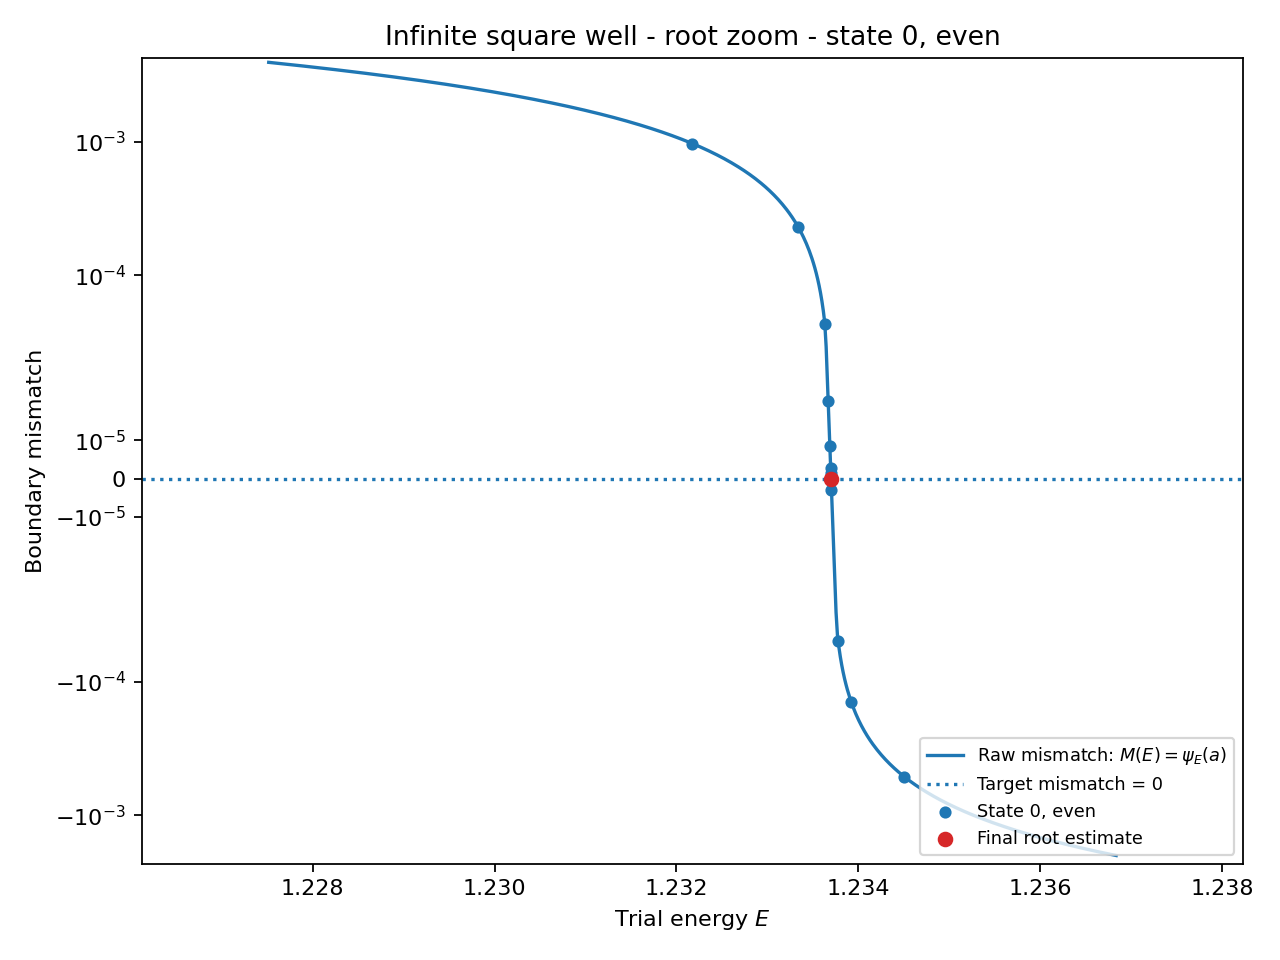
\includegraphics[height=5cm]{../../results/1_infinite_square_well_Numerov/1_infinite_square_well_Numerov_root_finding_state_0_even_zoom.png}
                        \caption{}
                    \end{subfigure}
                    \hfill
                    \begin{subfigure}[t]{0.485\textwidth}
                        \centering
                        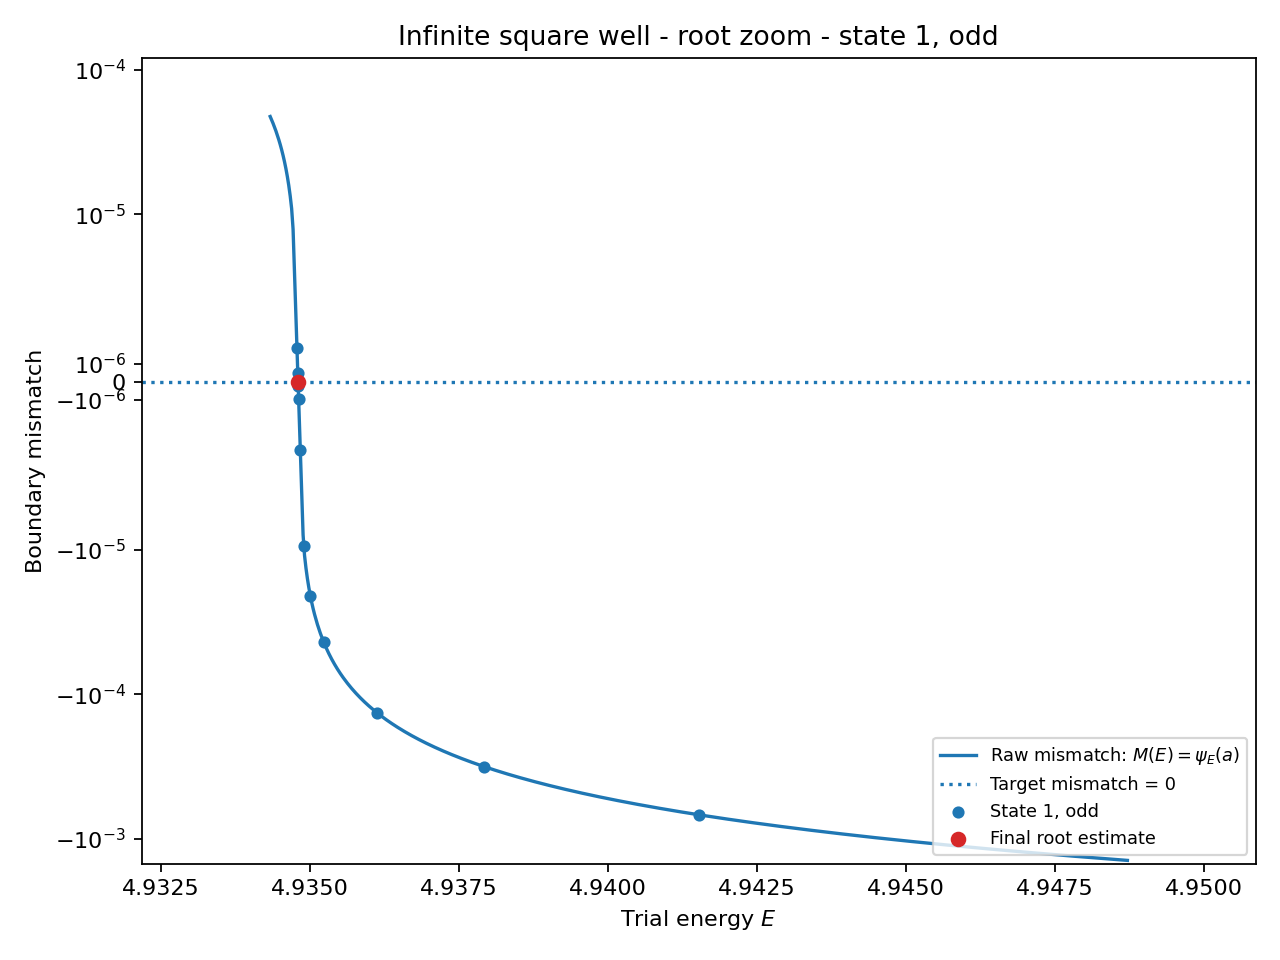
\includegraphics[height=5cm]{../../results/1_infinite_square_well_Numerov/1_infinite_square_well_Numerov_root_finding_state_1_odd_zoom.png}
                        \caption{}
                    \end{subfigure}

                    \captionof{figure}{Zoomed root brackets for the lowest even (a) and odd (b) infinite-well states. These panels show the raw mismatch only inside one initial sign-changing bracket, together with the recorded bisection iterates.}
                    \label{fig:infwell_shooting_zoom}
                \end{minipage}

                \vspace{1em}

                \begin{minipage}[t]{0.48\textwidth}
                    \centering
                    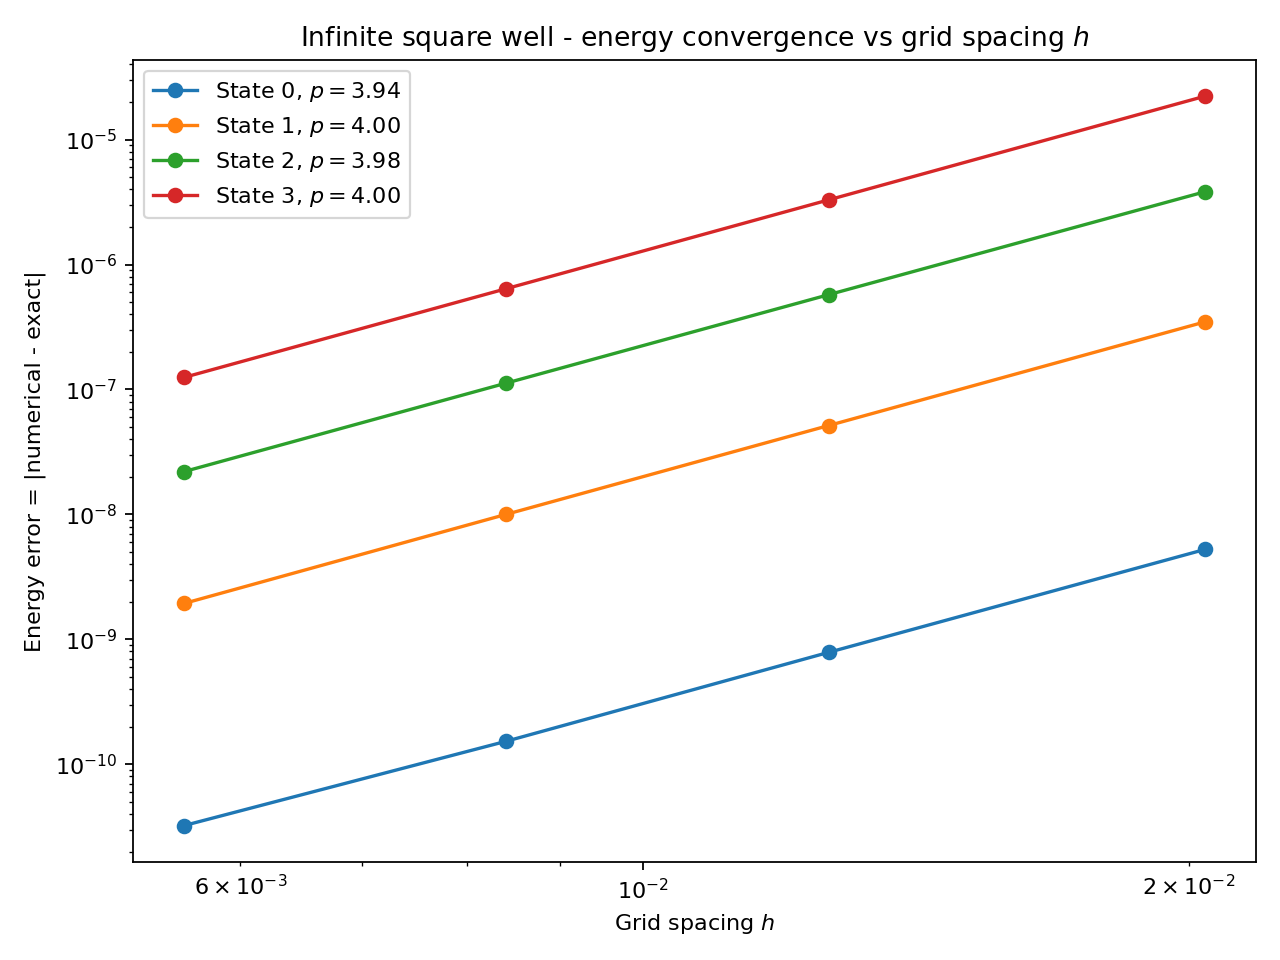
\includegraphics[width=\textwidth]{../../results/1_infinite_square_well_Numerov/1_infinite_square_well_Numerov_energy_convergence_vs_h.png}
                    \captionof{figure}{Convergence of the energy error as a function of grid spacing $h$. The slopes are close to fourth order, as expected for the Numerov method.}
                    \label{fig:infwell_convergence}
                \end{minipage}
                \hfill
                \begin{minipage}[t]{0.48\textwidth}
                    \centering
                    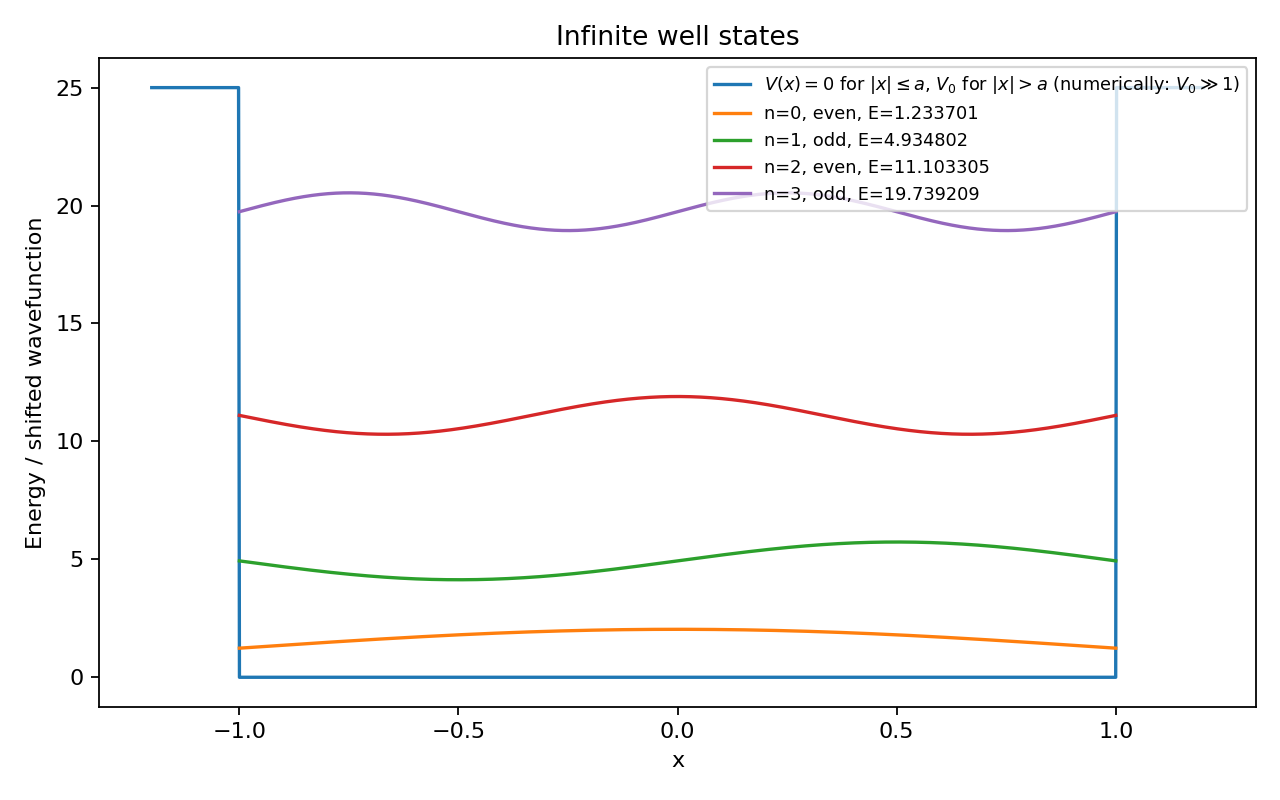
\includegraphics[width=\textwidth]{../../results/1_infinite_square_well_Numerov/1_infinite_square_well_Numerov_states.png}
                    \captionof{figure}{Wavefunctions for the first four states plotted together with their corresponding energies and the confining potential.}
                    \label{fig:infwell_states}
                \end{minipage}
            \end{figure}

        \subsection{Harmonic oscillator}
            \subsubsection{Numerov method on unbounded domains}
                For the harmonic oscillator with $V(x)=\tfrac{1}{2}\omega^2 x^2$, the exact spectrum is:
                \begin{equation}
                E_n = \omega\left(n+\tfrac{1}{2}\right), \qquad n=0,1,2,\ldots
                \end{equation}
                This provides a second analytic benchmark, but on an unbounded domain. Numerically, the domain is truncated to $[-x_{\max},x_{\max}]$, and decaying boundary conditions are imposed. In the production Numerov run, the parameters are $\omega=1$, $x_{\max}=8$, and $n_{\text{grid}}=2500$. The grid-convergence study uses $n_{\text{grid}}\in\{500,800,1200,1800,2500\}$ at fixed $x_{\max}=8$, while the box-size study uses $x_{\max}\in\{4,5,6,7,8,10\}$ at approximately fixed spacing. \\

                The numerical eigenvalues agree with the exact linear spectrum to extremely high precision, as shown in Fig.~\ref{fig:ho_energies}. In the saved run the first four relative errors are $6.2\times10^{-13}$, $2.3\times10^{-12}$, $6.6\times10^{-12}$, and $7.5\times10^{-12}$. This is exactly what should happen for the harmonic oscillator benchmark: the inward-shooting formulation suppresses contamination by the exponentially growing forbidden-region solution and cleanly recovers the exact ladder $E_n=\omega(n+\tfrac12)$. \\

                The probability densities (Fig.~\ref{fig:ho_densities}) show the expected structure: the ground state is centered and Gaussian-like, while the excited states alternate in parity and gain one additional node at each step. The support also broadens with increasing energy, consistent with the classical turning points moving outward. This confirms both physical correctness and stability of the integration on the truncated domain. \\

                The shooting mismatch functions (Fig.~\ref{fig:ho_shooting}) exhibit clear zero crossings at the expected energies. In the even sector the roots lie near $E\approx0.5$ and $E\approx2.5$, while in the odd sector they lie near $E\approx1.5$ and $E\approx3.5$. The raw mismatch spans many orders of magnitude because the inward integration starts in the decaying tail, but the sign changes remain sharp and the roots alternate even--odd as they should. The corresponding zoomed brackets in Fig.~\ref{fig:ho_shooting_zoom} make that local sign change explicit and show the final bisection convergence in the neighborhood of a single root rather than over the full dynamic range of the scan. \\

                Convergence with respect to grid spacing $h$ (Fig.~\ref{fig:ho_convergence_h}) is overall consistent with fourth-order behavior. The saved study gives fitted slopes $p\approx5.30$, $3.97$, $4.57$, and $4.00$ for the first four states. The two slopes above four are not evidence of true superconvergence: they occur only after the errors have already dropped to the $10^{-11}$--$10^{-12}$ range, where root-finding tolerance and floating-point effects distort a short log--log fit. The raw errors themselves still decrease in the expected high-order way, from about $3.2\times10^{-9}$--$2.6\times10^{-8}$ on the coarsest grid to $5.1\times10^{-13}$--$2.6\times10^{-11}$ on the finest grid. \\

                The dependence on domain size in Fig.~\ref{fig:ho_convergence_xmax} shows the expected truncation-to-discretization crossover. At $x_{\max}=4$ the tail is clipped too aggressively and the fourth-state error is still about $5.9\times10^{-5}$. By $x_{\max}=5$ the errors have already fallen dramatically, and by $x_{\max}\approx6$ the curves flatten near the discretization floor: roughly $10^{-12}$ for the ground state, a few $10^{-12}$ for the first odd state, and about $10^{-11}$--$10^{-10}$ for the higher states. This confirms that the dominant error for large boxes is no longer domain truncation. \\

                Finally, the combined state plot (Fig.~\ref{fig:ho_states}) shows the wavefunctions together with the confining potential. The increasing spatial extent and alternating parity agree with the analytic harmonic-oscillator picture. \\

                \begin{figure}[p]
                    \centering

                    \begin{minipage}[t]{0.48\textwidth}
                        \centering
                        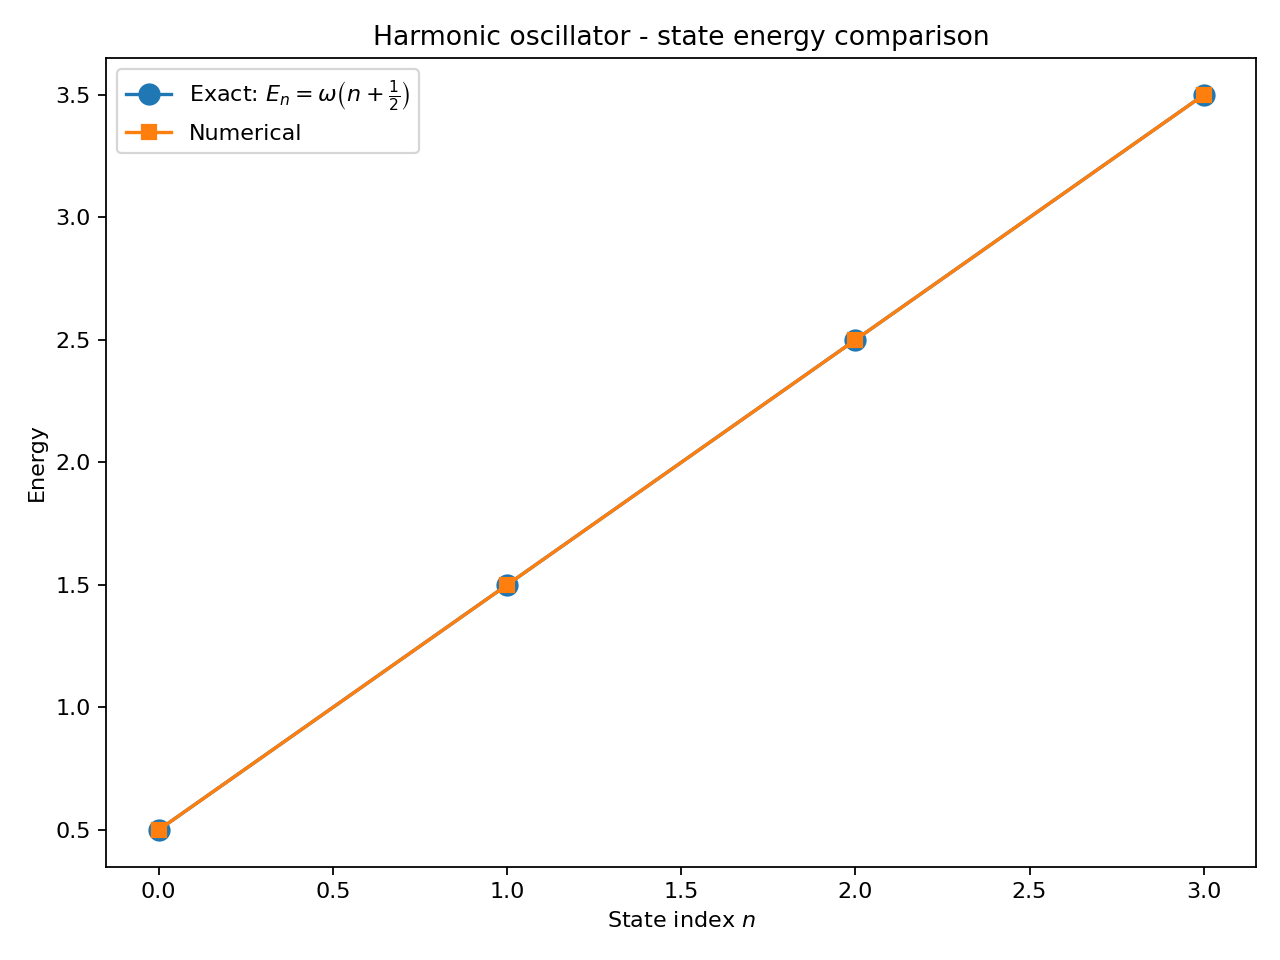
\includegraphics[width=\textwidth]{../../results/2a_harmonic_oscillator_Numerov/2a_harmonic_oscillator_Numerov_state_energy_comparison.png}
                        \captionof{figure}{Comparison between numerical and exact energy eigenvalues for the harmonic oscillator. The agreement is excellent for the first four states.}
                        \label{fig:ho_energies}
                    \end{minipage}
                    \hfill
                    \begin{minipage}[t]{0.48\textwidth}
                        \centering
                        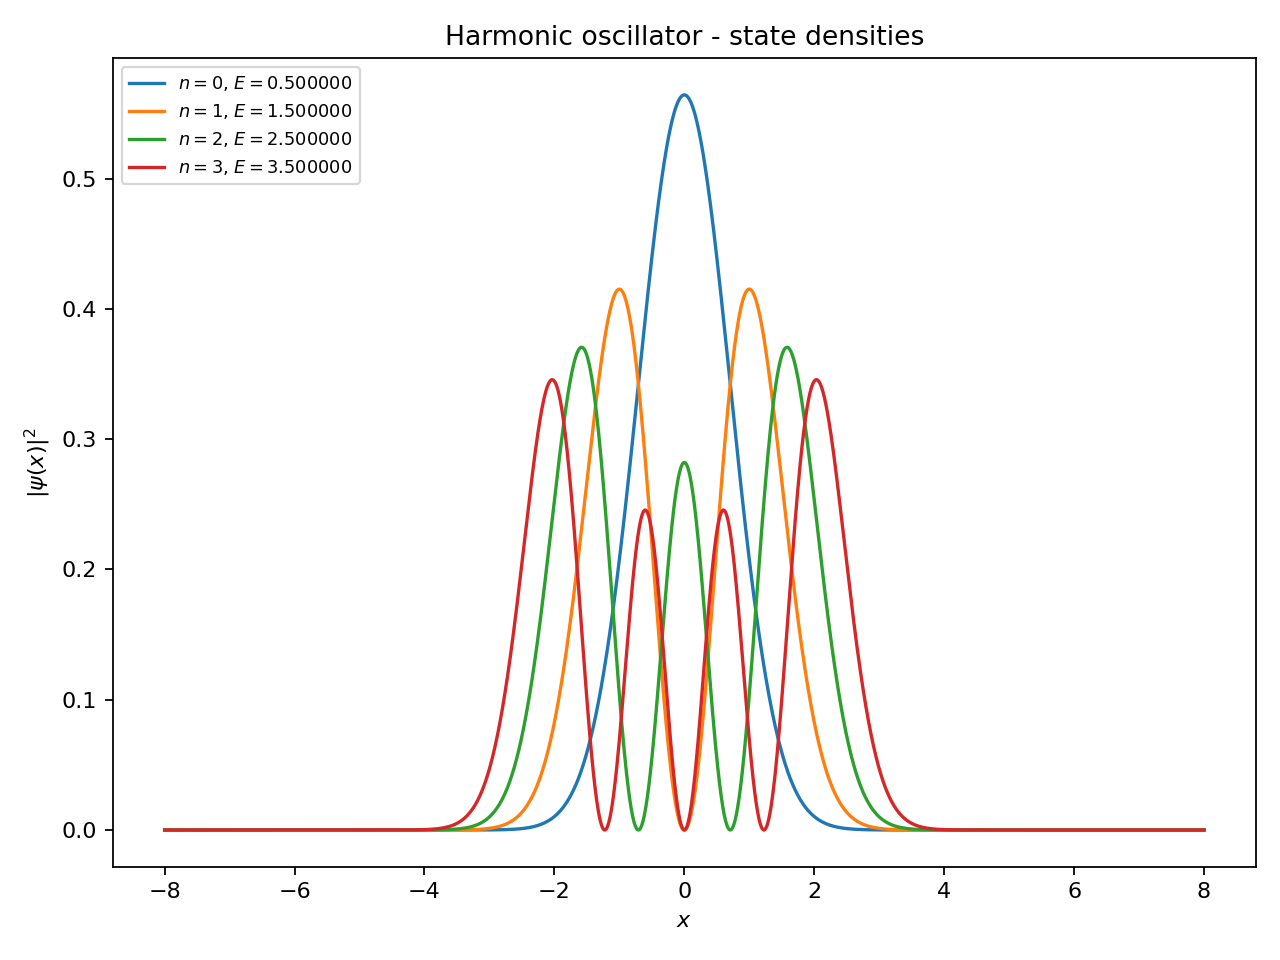
\includegraphics[width=\textwidth]{../../results/2a_harmonic_oscillator_Numerov/2a_harmonic_oscillator_Numerov_state_densities.png}
                        \captionof{figure}{Probability densities $|\psi(x)|^2$ for the first four harmonic oscillator eigenstates. The correct node structure is clearly reproduced.}
                        \label{fig:ho_densities}
                    \end{minipage}

                    \vspace{1em}

                    \begin{minipage}[t]{\textwidth}
                        \centering
                        \begin{subfigure}[t]{0.485\textwidth}
                            \centering
                            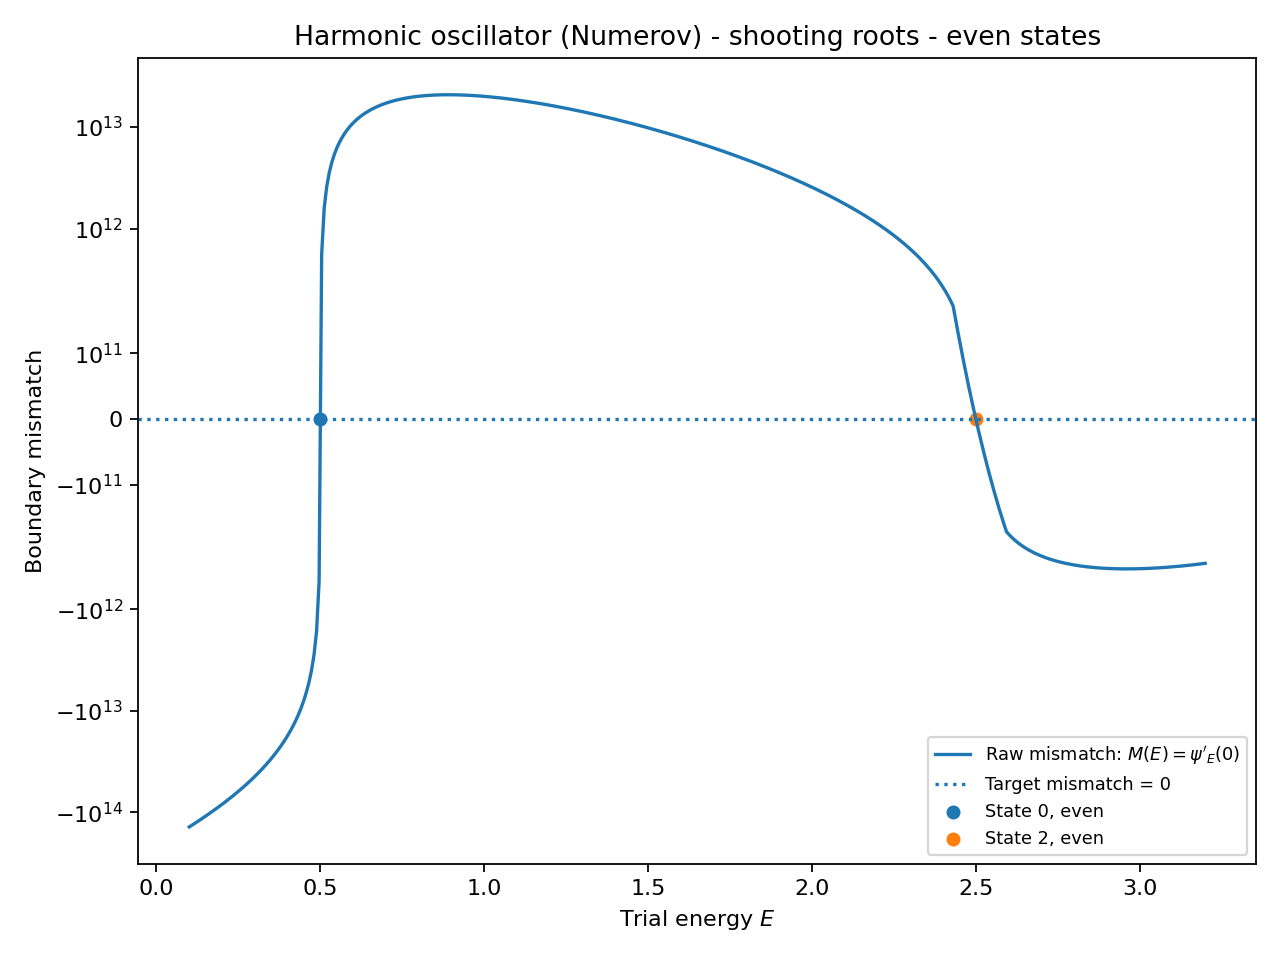
\includegraphics[height=5cm]{../../results/2a_harmonic_oscillator_Numerov/2a_harmonic_oscillator_Numerov_root_finding_even.png}
                            \caption{}
                        \end{subfigure}
                        \hfill
                        \begin{subfigure}[t]{0.485\textwidth}
                            \centering
                            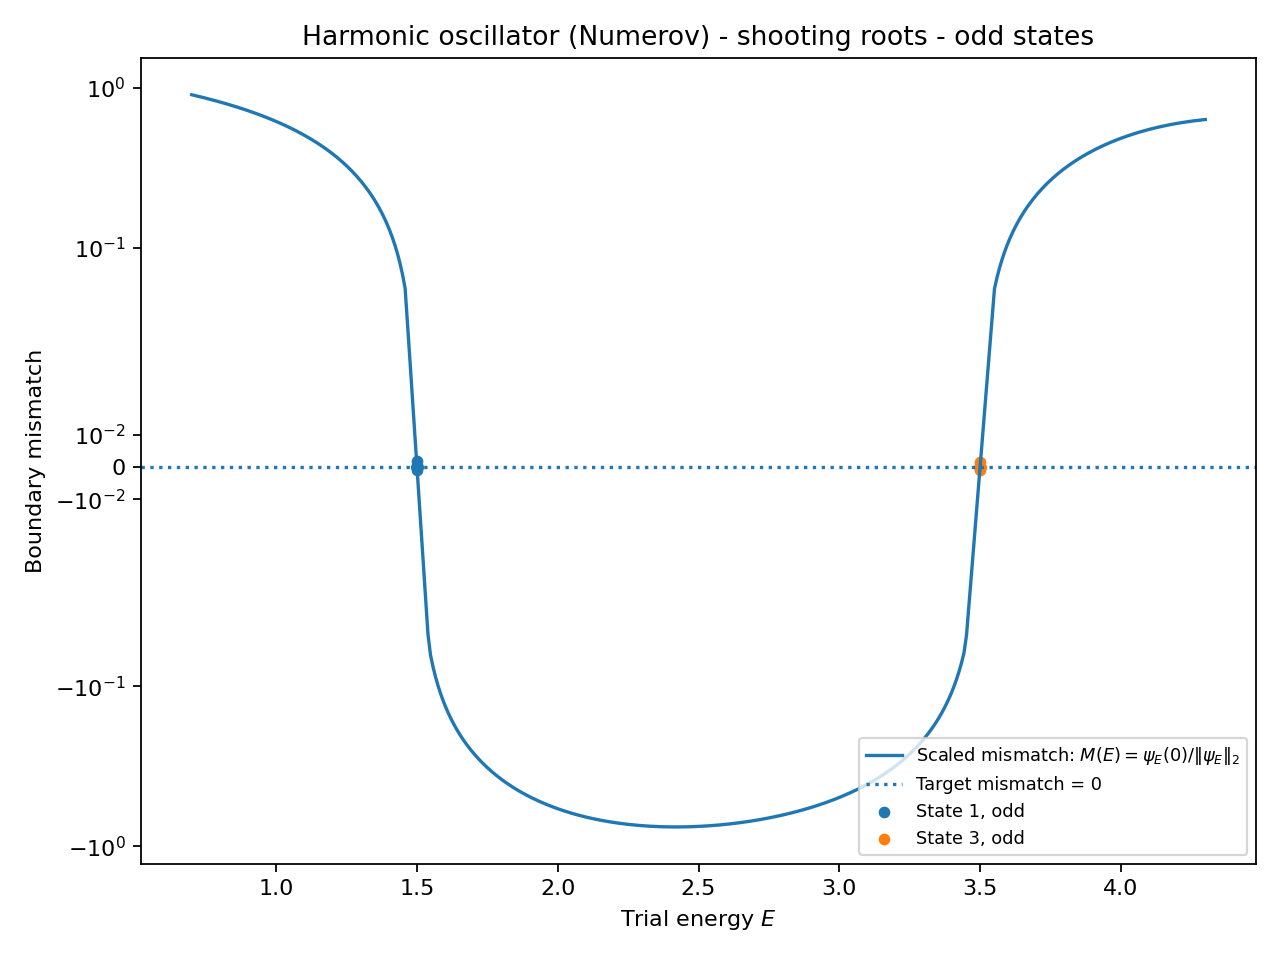
\includegraphics[height=5cm]{../../results/2a_harmonic_oscillator_Numerov/2a_harmonic_oscillator_Numerov_root_finding_odd.png}
                            \caption{}
                        \end{subfigure}

                        \captionof{figure}{Raw boundary mismatch functions for even (a) and odd (b) states. The zero crossings correspond to the physical eigenvalues.}
                        \label{fig:ho_shooting}
                    \end{minipage}

                    \vspace{1em}

                    \begin{minipage}[t]{\textwidth}
                        \centering
                        \begin{subfigure}[t]{0.485\textwidth}
                            \centering
                            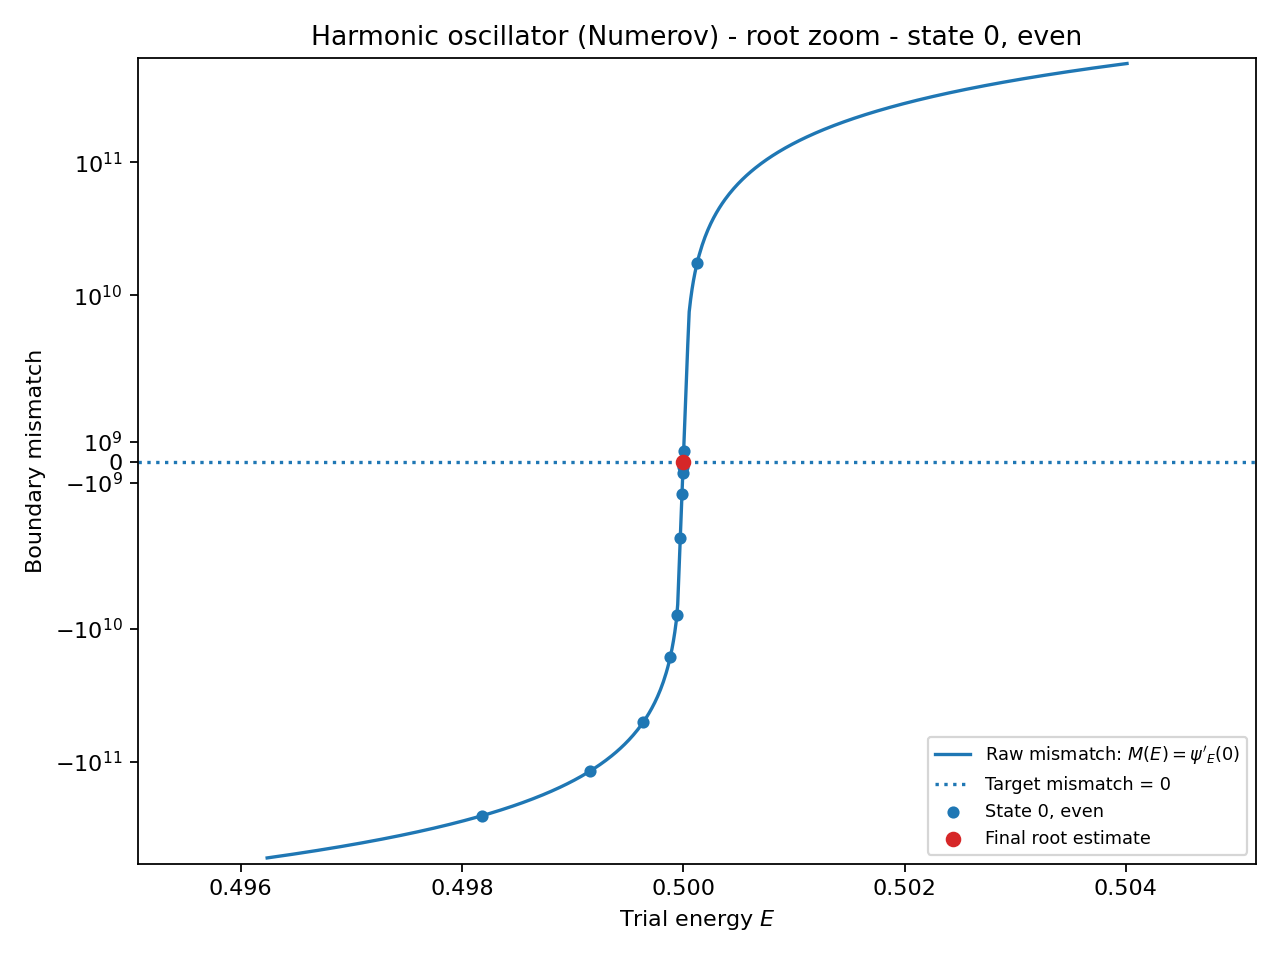
\includegraphics[height=5cm]{../../results/2a_harmonic_oscillator_Numerov/2a_harmonic_oscillator_Numerov_root_finding_state_0_even_zoom.png}
                            \caption{}
                        \end{subfigure}
                        \hfill
                        \begin{subfigure}[t]{0.485\textwidth}
                            \centering
                            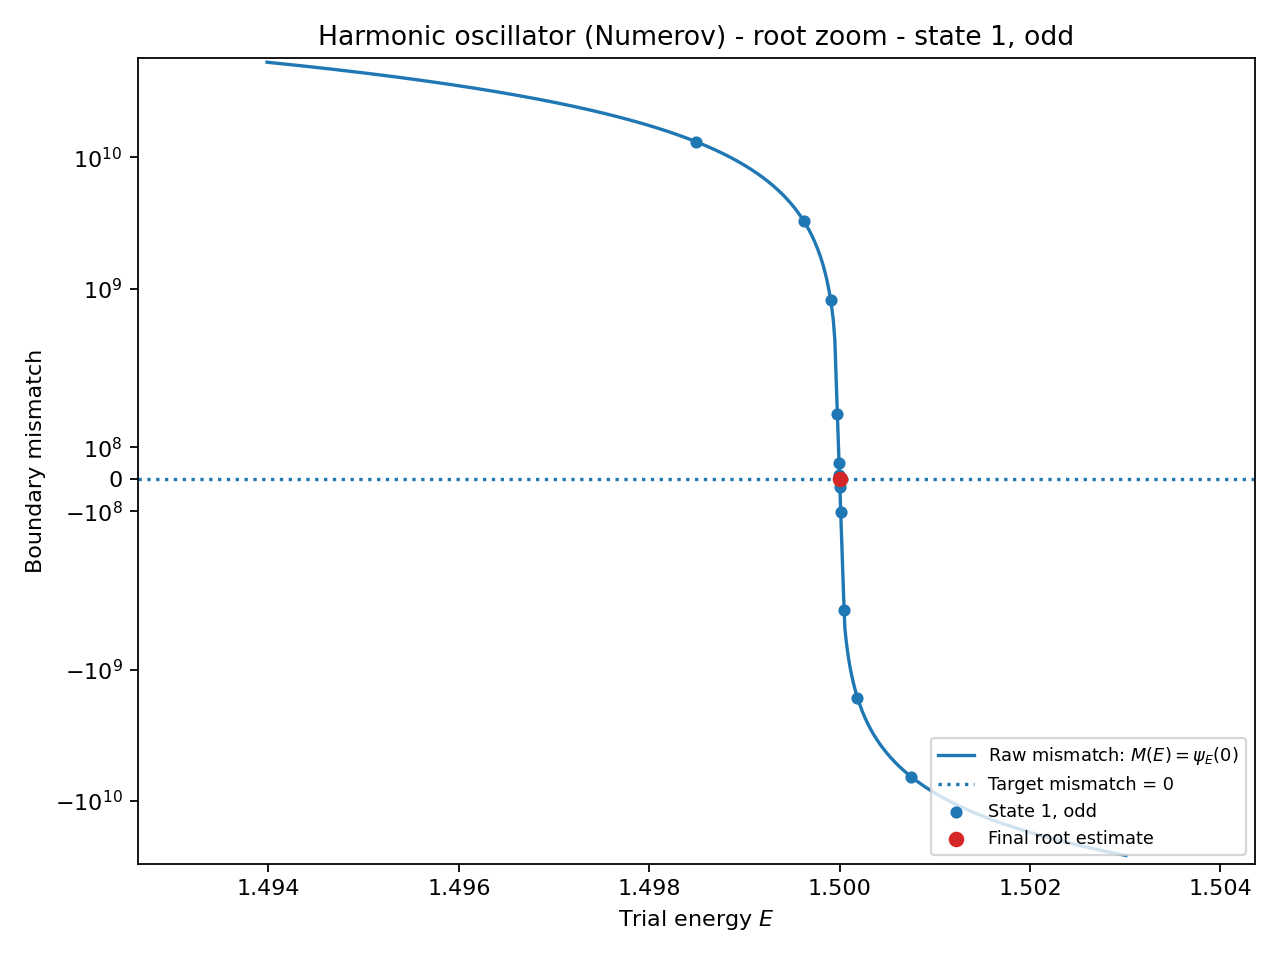
\includegraphics[height=5cm]{../../results/2a_harmonic_oscillator_Numerov/2a_harmonic_oscillator_Numerov_root_finding_state_1_odd_zoom.png}
                            \caption{}
                        \end{subfigure}

                        \captionof{figure}{Zoomed root brackets for the lowest even (a) and odd (b) harmonic-oscillator states. These local views remove the global dynamic-range compression and show the raw mismatch together with the bisection iterates inside each initial bracket.}
                        \label{fig:ho_shooting_zoom}
                    \end{minipage}
                \end{figure}

                \begin{figure}[p]
                    \centering

                    \begin{minipage}[t]{0.48\textwidth}
                        \centering
                        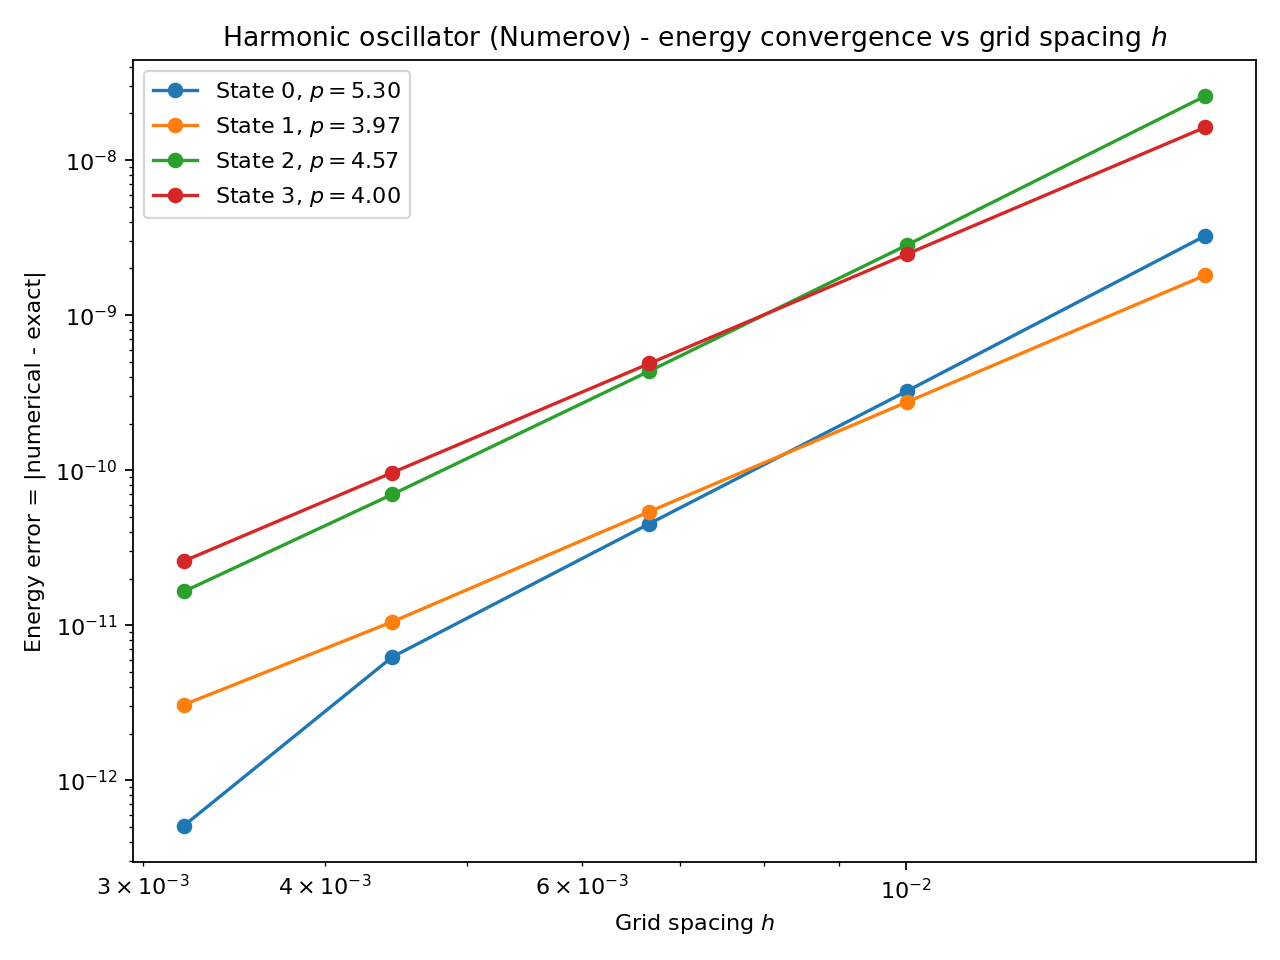
\includegraphics[width=\textwidth]{../../results/2a_harmonic_oscillator_Numerov/2a_harmonic_oscillator_Numerov_energy_convergence_vs_h.png}
                        \captionof{figure}{Convergence of the energy error as a function of grid spacing $h$. The slopes are close to fourth order, as expected for the Numerov method.}
                        \label{fig:ho_convergence_h}
                    \end{minipage}
                    \hfill
                    \begin{minipage}[t]{0.48\textwidth}
                        \centering
                        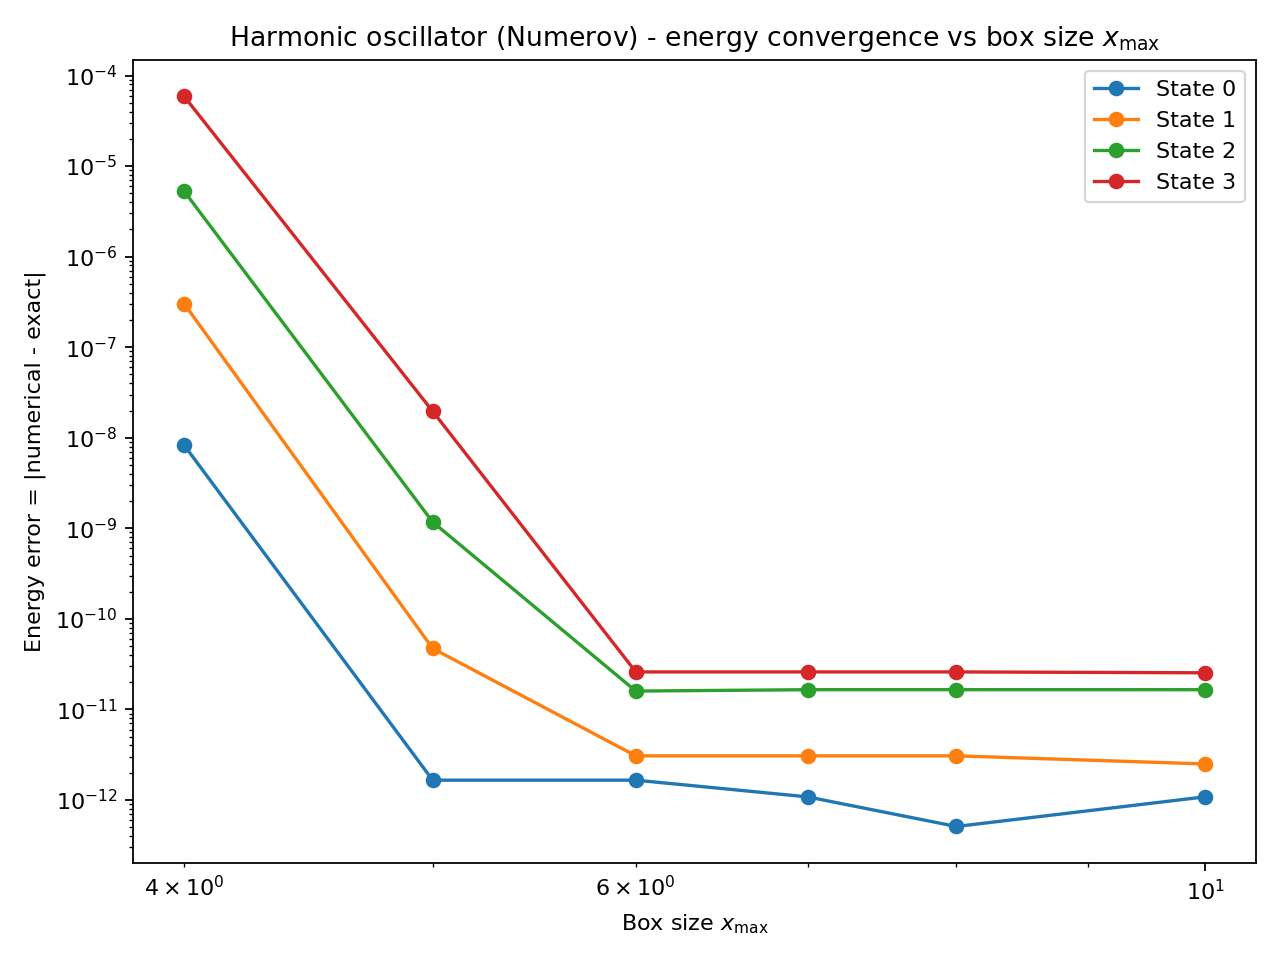
\includegraphics[width=\textwidth]{../../results/2a_harmonic_oscillator_Numerov/2a_harmonic_oscillator_Numerov_energy_convergence_vs_x_max.png}
                        \captionof{figure}{Dependence of the energy error on the domain size $x_{\max}$. Errors decrease rapidly before reaching a plateau set by discretization and floating-point limits.}
                        \label{fig:ho_convergence_xmax}
                    \end{minipage}

                    \vspace{1em}

                    \begin{minipage}[t]{0.48\textwidth}
                        \centering
                        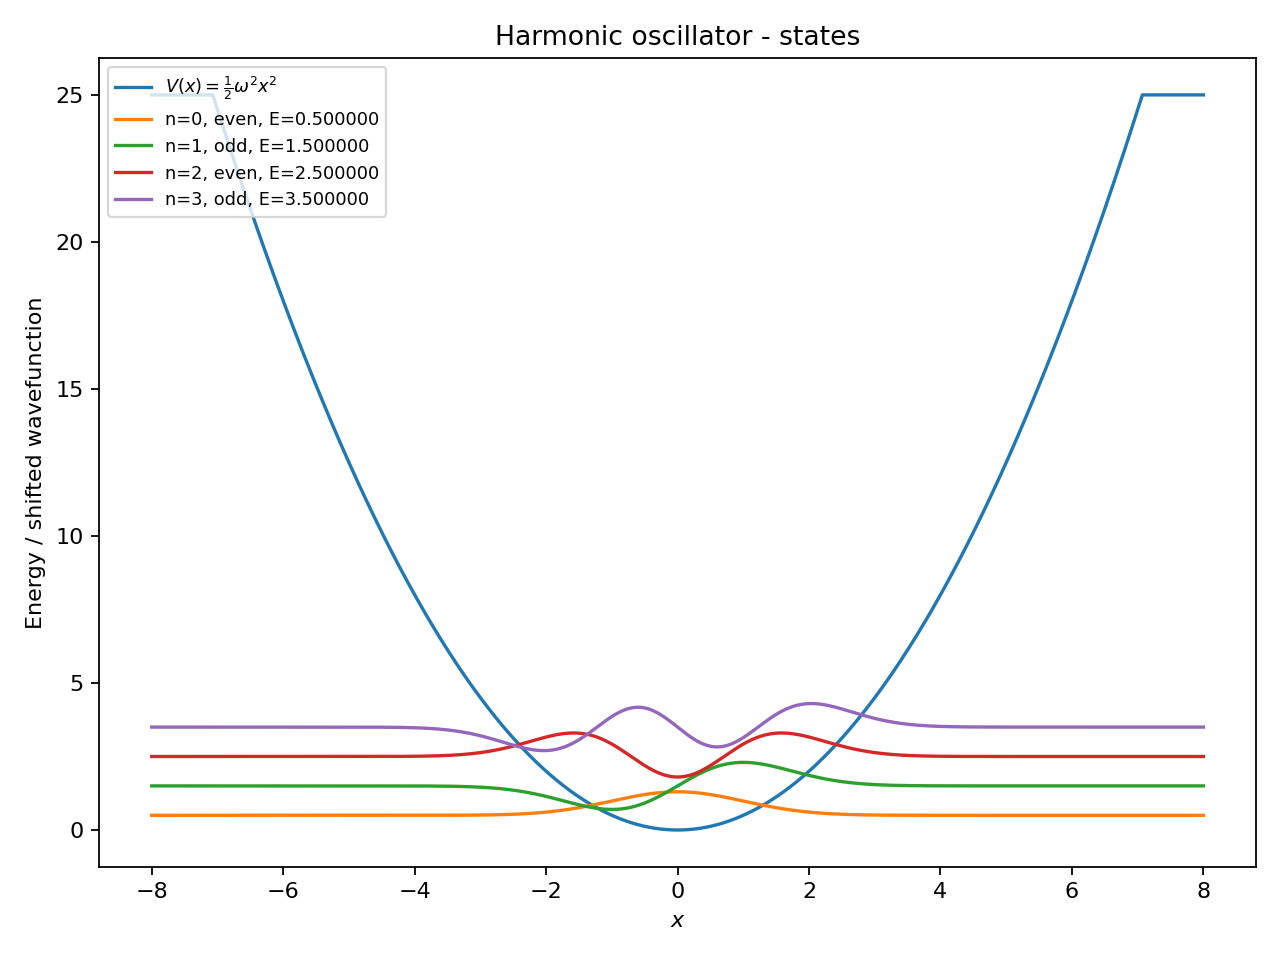
\includegraphics[width=\textwidth]{../../results/2a_harmonic_oscillator_Numerov/2a_harmonic_oscillator_Numerov_states.png}
                        \captionof{figure}{Wavefunctions for the first four harmonic oscillator states plotted together with the potential.}
                        \label{fig:ho_states}
                    \end{minipage}
                    \hfill
                    \begin{minipage}[t]{0.48\textwidth}
                        \centering
                        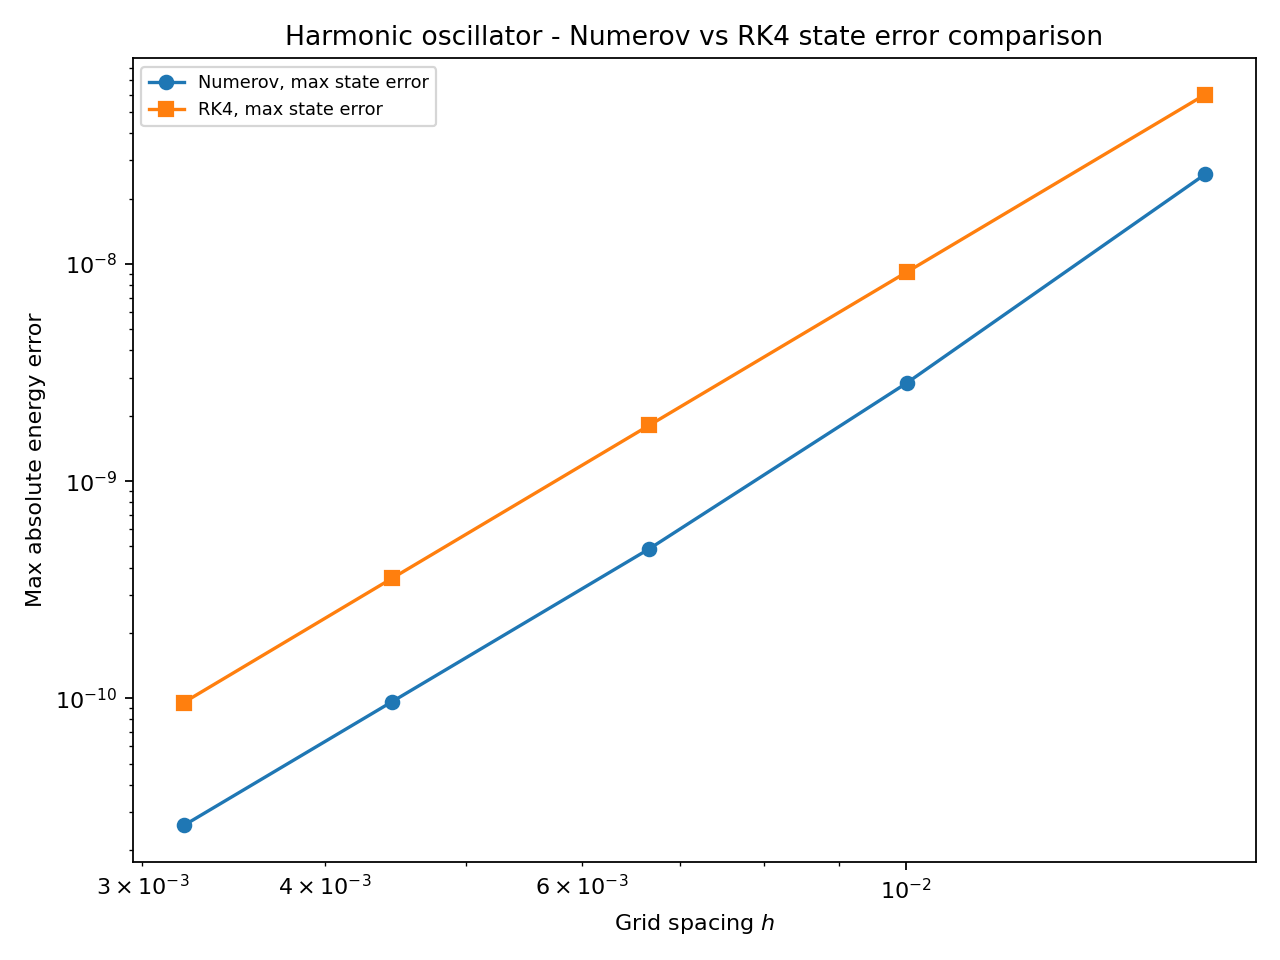
\includegraphics[width=\textwidth]{../../results/2c_harmonic_oscillator_Numerov_VS_RK4_comparison/2c_harmonic_oscillator_Numerov_VS_RK4_state_error_comparison.png}
                        \captionof{figure}{Comparison of Numerov and RK4 shooting for the harmonic oscillator. Both methods show fourth-order convergence, while Numerov gives a smaller maximum energy error at the same grid spacing.}
                        \label{fig:ho_numerov_vs_rk4}
                    \end{minipage}
                \end{figure}

            \subsubsection{Numerov versus Runge--Kutta}
                As an additional method comparison, the harmonic oscillator was also solved using a fourth-order Runge--Kutta (RK4) shooting method. In this formulation the second-order Schr\"odinger equation is rewritten as the first-order system:
                \begin{equation}
                \psi' = \phi, \qquad
                \phi' = 2[V(x)-E]\psi
                \end{equation}
                This makes RK4 a useful general-purpose comparison for Numerov, which instead exploits the special second-order structure of the Schr\"odinger equation directly. The RK4 comparison uses the same physical parameters $\omega=1$ and $x_{\max}=8$ as the Numerov run, and it reuses the same family of grid spacings derived from the Numerov convergence study so the two methods are compared on matched meshes. The representative RK4 spectrum plot uses $n_{\text{grid}}=1200$, and the RK4 box-size study again takes $x_{\max}\in\{4,5,6,7,8,10\}$ at approximately fixed spacing. \\

                Figure~\ref{fig:ho_numerov_vs_rk4} compares the maximum energy error over the computed harmonic-oscillator states as a function of grid spacing. Both methods show approximately fourth-order convergence, as expected. The RK4 slopes are much more uniformly close to four than the Numerov fit, with saved values $p\approx4.04$, $4.02$, $4.01$, and $4.00$. On the saved grids, the maximum absolute error ranges from $2.6\times10^{-8}$ down to $2.6\times10^{-11}$ for Numerov and from $6.0\times10^{-8}$ down to $9.6\times10^{-11}$ for RK4, so Numerov is consistently better by a factor of about $2$--$4$ at fixed $h$ even though both methods are fourth order. \\

                The box-size study tells the same story for both methods. At fixed spacing, increasing $x_{\max}$ from $4$ to $6$ sharply reduces the truncation error, after which both methods level off at their respective discretization floors. This is a useful reminder that method order alone is not the whole story: domain truncation, root-finding tolerance, and boundary diagnostics all matter. After using a high-order boundary derivative for the Numerov inward-shooting condition, the Numerov and RK4 comparison behaves as expected and gives Numerov the smaller error at matched grid spacing.

        \subsection{Double-well potential}
            The quartic double-well potential is used as the main nontrivial bound-state example. In the shifted form used here:
            \begin{equation}
            V(x)=ax^4-bx^2-V_{\min}, \qquad V_{\min}=-\frac{b^2}{4a}
            \end{equation}
            the two minima are shifted to zero. Unlike the infinite square well and harmonic oscillator, this system does not have a simple analytic spectrum, so the validation relies on internal consistency checks, convergence studies, parity structure, and physically expected tunneling behavior. The production run uses $a=1$, $b=6$, the analytic minimum shift $V_{\min}=b^2/(4a)$, a box size $x_{\max}=4$, and $n_{\text{grid}}=4000$. The successive-refinement study uses $n_{\text{grid}}\in\{600,1000,1600,2200,3000,4000\}$, the box-size study uses $x_{\max}\in\{2.5,3.0,3.5,4.0,4.5,5.0\}$ at approximately fixed spacing, and the splitting sweep varies $b\in\{3,4,5,6,7,8\}$ with $a=1$. \\

            Figure~\ref{fig:dw_states} shows the first four computed states together with the double-well potential. The two lowest states form a nearly degenerate even-odd pair, with energies $E_0\approx2.357273$ and $E_1\approx2.359372$, so the splitting is only about $2.10\times10^{-3}$. This is the expected tunneling doublet: the even and odd states are symmetric and antisymmetric combinations of states localized in the two wells. The next pair is much higher in energy, with $E_2\approx6.548814$ and $E_3\approx6.684430$, and its splitting is much larger because those states overlap more strongly through the central barrier. \\

            The probability densities in Fig.~\ref{fig:dw_densities} show the expected localization near the two wells. The lowest pair has nearly identical density, because the sign difference between even and odd wavefunctions disappears in $|\psi(x)|^2$. The higher states show additional node structure and broader support, as expected for excited double-well states. The figure also makes the tunneling interpretation concrete: the low-lying states are concentrated in the two minima near $x=\pm\sqrt{b/2}$, while the barrier region near the origin is sampled only through the small connecting tail. \\

            The root-finding diagnostics (Fig.~\ref{fig:dw_shooting}) show well-defined zero crossings in the even and odd parity sectors. For the saved run, the first even-sector roots occur near $E\approx2.36$ and $E\approx6.55$, while the first odd-sector roots occur near $E\approx2.36$ and $E\approx6.68$. The corresponding zoom views in Fig.~\ref{fig:dw_shooting_zoom} confirm that these are genuine local sign changes of the raw mismatch and not artifacts of the large boundary amplitudes seen in the full scan. \\

            Since there is no closed-form exact spectrum for this potential, grid convergence is measured using successive refinements at fixed domain size. The convergence with respect to grid spacing (Fig.~\ref{fig:dw_convergence_h}) still shows stable high-order behavior, with fitted slopes $p\approx4.18$, $3.95$, $4.55$, and $5.67$ for the first four states. The values above four should not be overinterpreted as true superconvergence. They appear only when the successive-difference errors have already fallen to about $10^{-12}$--$10^{-13}$ for the low states and $10^{-11}$ for the higher states, so short log--log fits are being distorted by the numerical floor. What matters physically is that every state improves systematically under refinement and the dominant trend remains high-order decay of the error. \\

            The box-size study (Fig.~\ref{fig:dw_convergence_xmax}) shows an especially important numerical effect for this problem. At $x_{\max}=2.5$ the box is clearly too small: the errors are still of order $10^{-1}$. At $x_{\max}=3.0$ they have dropped to the $10^{-4}$--$10^{-3}$ range, and by $x_{\max}=3.5$ they are already down near $10^{-8}$. Once the box reaches $x_{\max}\approx4.0$, the remaining error is only about $10^{-12}$ relative to the larger-box reference, so the final reported states are no longer dominated by artificial boundary truncation. This is exactly why the production calculation uses a larger box than the earlier, visibly contaminated small-box runs. \\

            Finally, Fig.~\ref{fig:dw_splitting} shows how the lowest even-odd splitting changes with the double-well parameter $b$. As $b$ increases from $3$ to $8$, the splitting falls from about $3.52\times10^{-1}$ to $1.59\times10^{-5}$. This is the expected physical signature of tunneling suppression: increasing $b$ deepens and separates the wells, raises the effective barrier between them, and therefore reduces the overlap between the left- and right-localized components. \\

            Overall, the double-well results demonstrate that the solver works beyond analytic benchmarks. The computed states have the expected parity, localization, and near-degenerate tunneling structure; the splitting with respect to $b$ behaves physically; and the convergence studies show that the numerical results are stable with respect to both grid spacing and domain size once the computational box is chosen large enough. \\

            \begin{figure}[p]
                \centering

                \begin{minipage}[t]{0.48\textwidth}
                    \centering
                    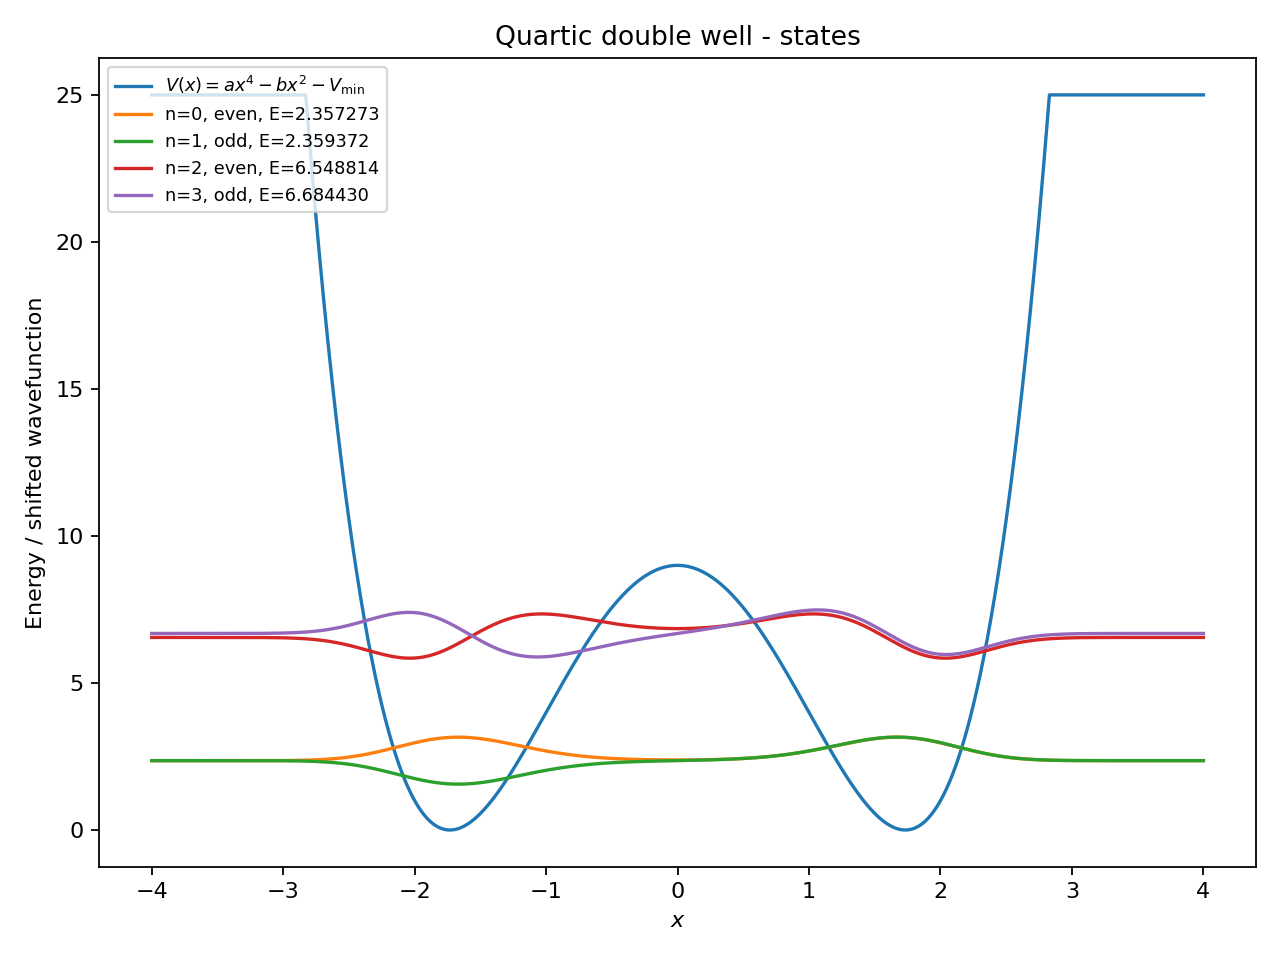
\includegraphics[width=\textwidth]{../../results/3_double_well_Numerov/3_double_well_Numerov_states.png}
                    \captionof{figure}{First four bound states of the quartic double-well potential. The lowest two states form a nearly degenerate tunneling doublet.}
                    \label{fig:dw_states}
                \end{minipage}
                \hfill
                \begin{minipage}[t]{0.48\textwidth}
                    \centering
                    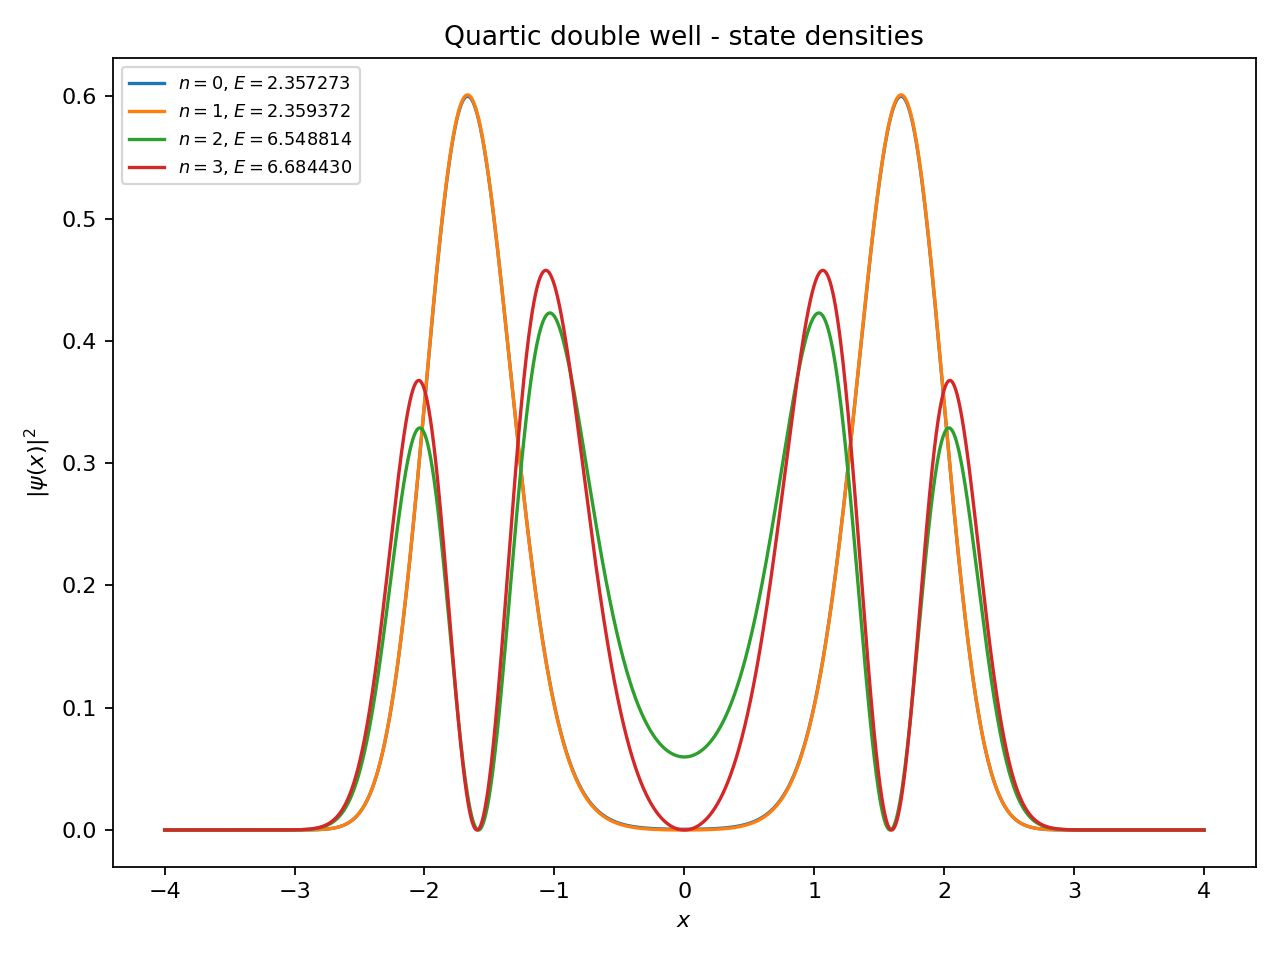
\includegraphics[width=\textwidth]{../../results/3_double_well_Numerov/3_double_well_Numerov_state_densities.png}
                    \captionof{figure}{Probability densities $|\psi(x)|^2$ for the first four double-well states. The lowest even and odd states have nearly identical densities, as expected for a tunneling doublet.}
                    \label{fig:dw_densities}
                \end{minipage}

                \vspace{1em}

                \begin{minipage}[t]{\textwidth}
                    \centering
                    \begin{subfigure}[t]{0.485\textwidth}
                        \centering
                        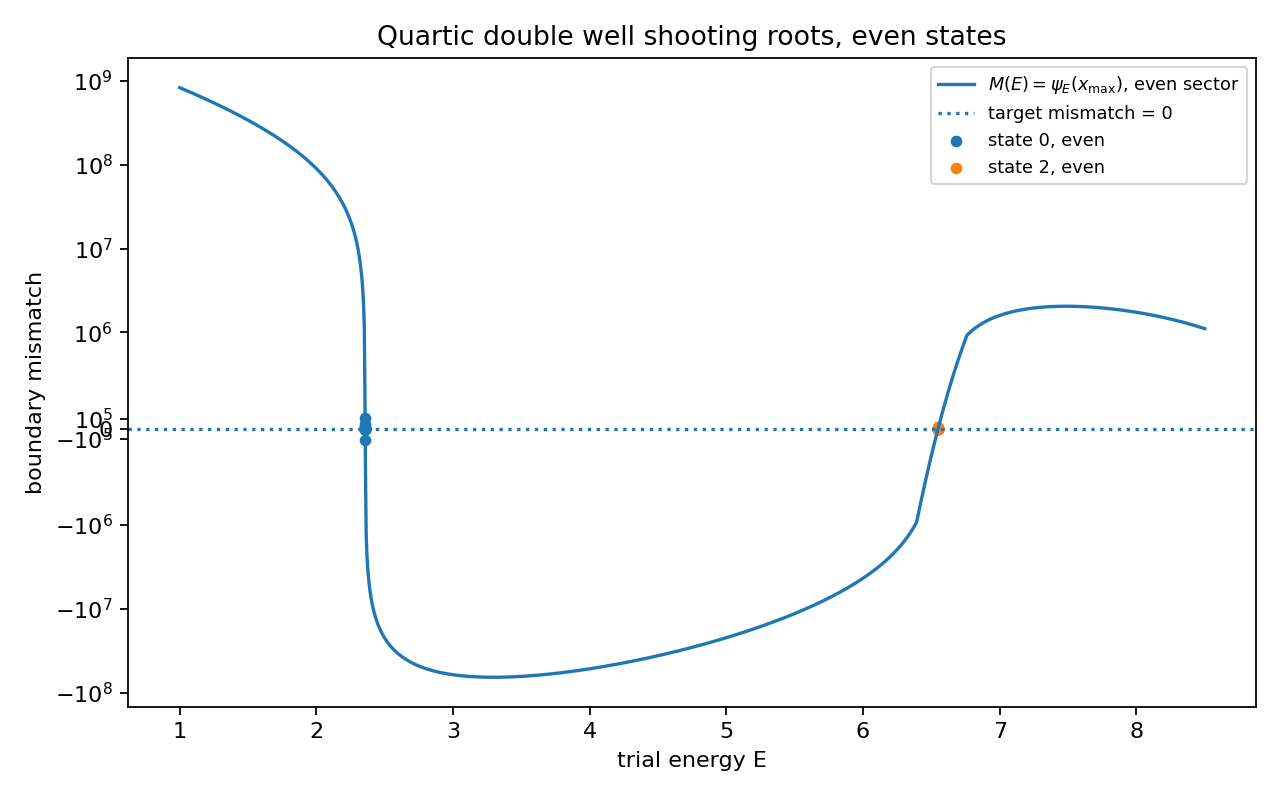
\includegraphics[height=5cm]{../../results/3_double_well_Numerov/3_double_well_Numerov_root_finding_even.png}
                        \caption{}
                    \end{subfigure}
                    \hfill
                    \begin{subfigure}[t]{0.485\textwidth}
                        \centering
                        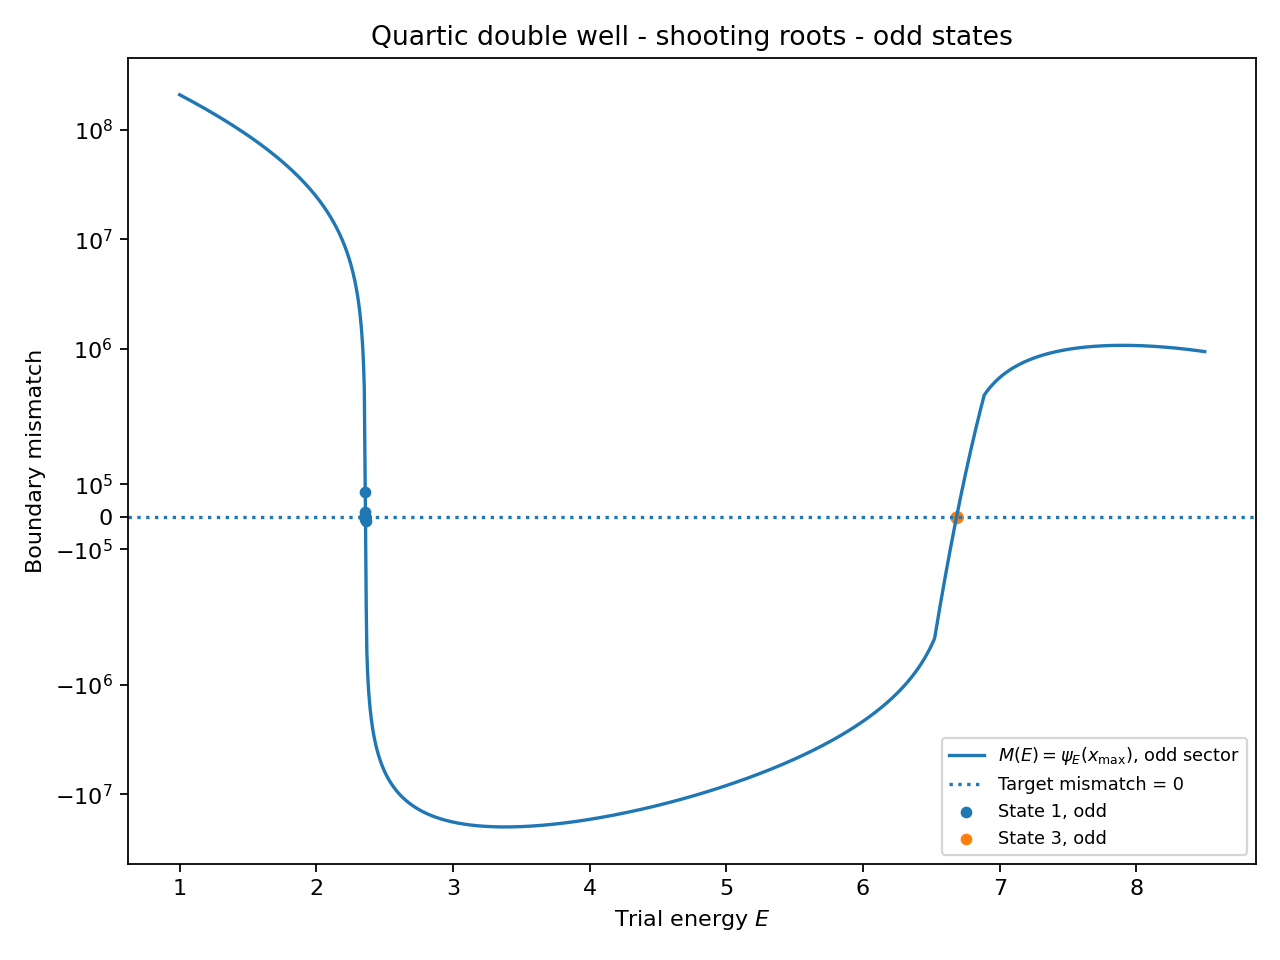
\includegraphics[height=5cm]{../../results/3_double_well_Numerov/3_double_well_Numerov_root_finding_odd.png}
                        \caption{}
                    \end{subfigure}

                    \captionof{figure}{Raw shooting mismatch functions for even (top) and odd (bottom) double-well states. The zero crossings define the numerical eigenvalues.}
                    \label{fig:dw_shooting}
                \end{minipage}

                \vspace{1em}

                \begin{minipage}[t]{\textwidth}
                    \centering
                    \begin{subfigure}[t]{0.485\textwidth}
                        \centering
                        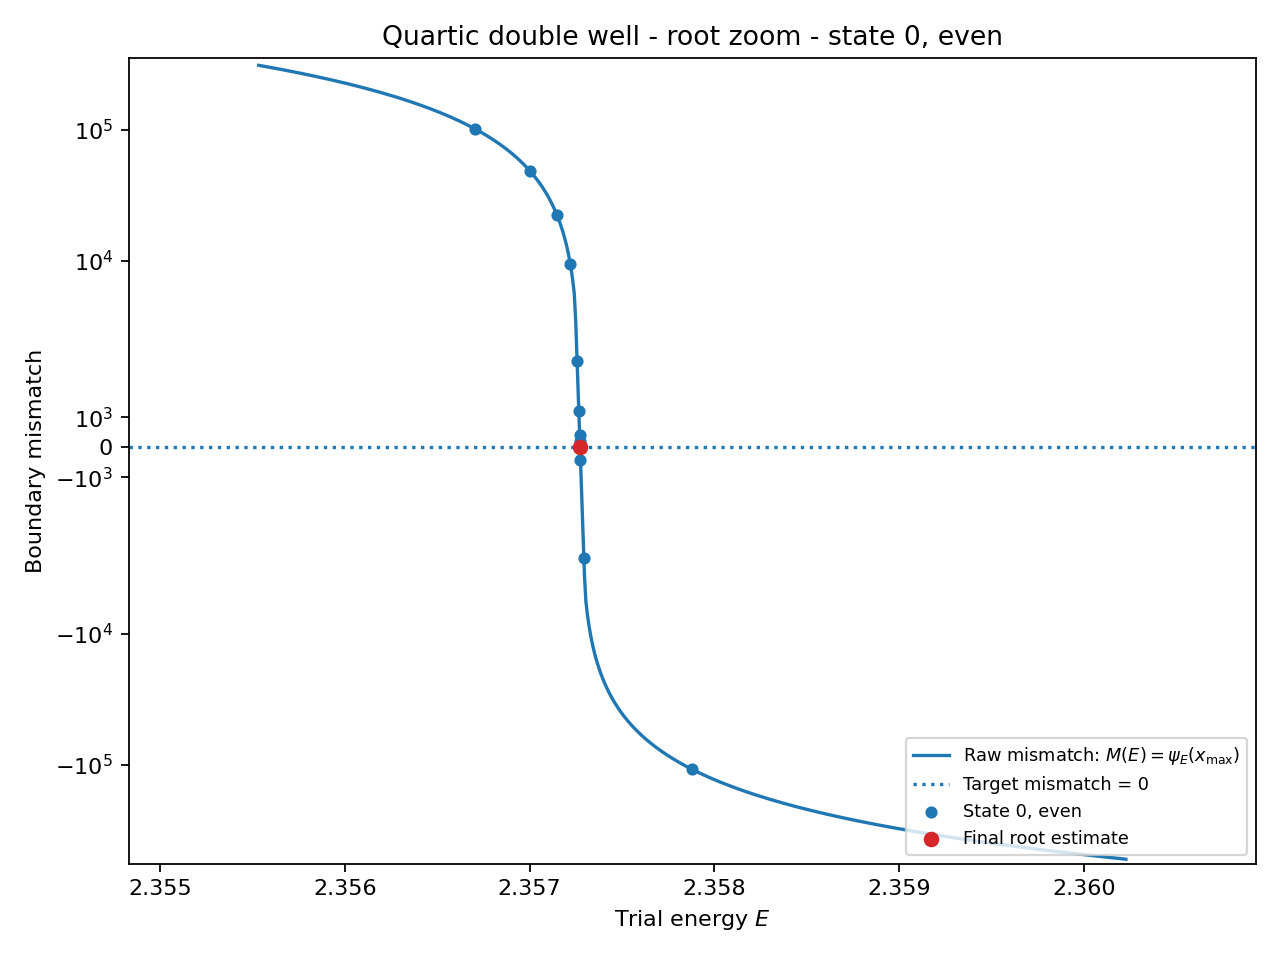
\includegraphics[height=5cm]{../../results/3_double_well_Numerov/3_double_well_Numerov_root_finding_state_0_even_zoom.png}
                        \caption{}
                    \end{subfigure}
                    \hfill
                    \begin{subfigure}[t]{0.485\textwidth}
                        \centering
                        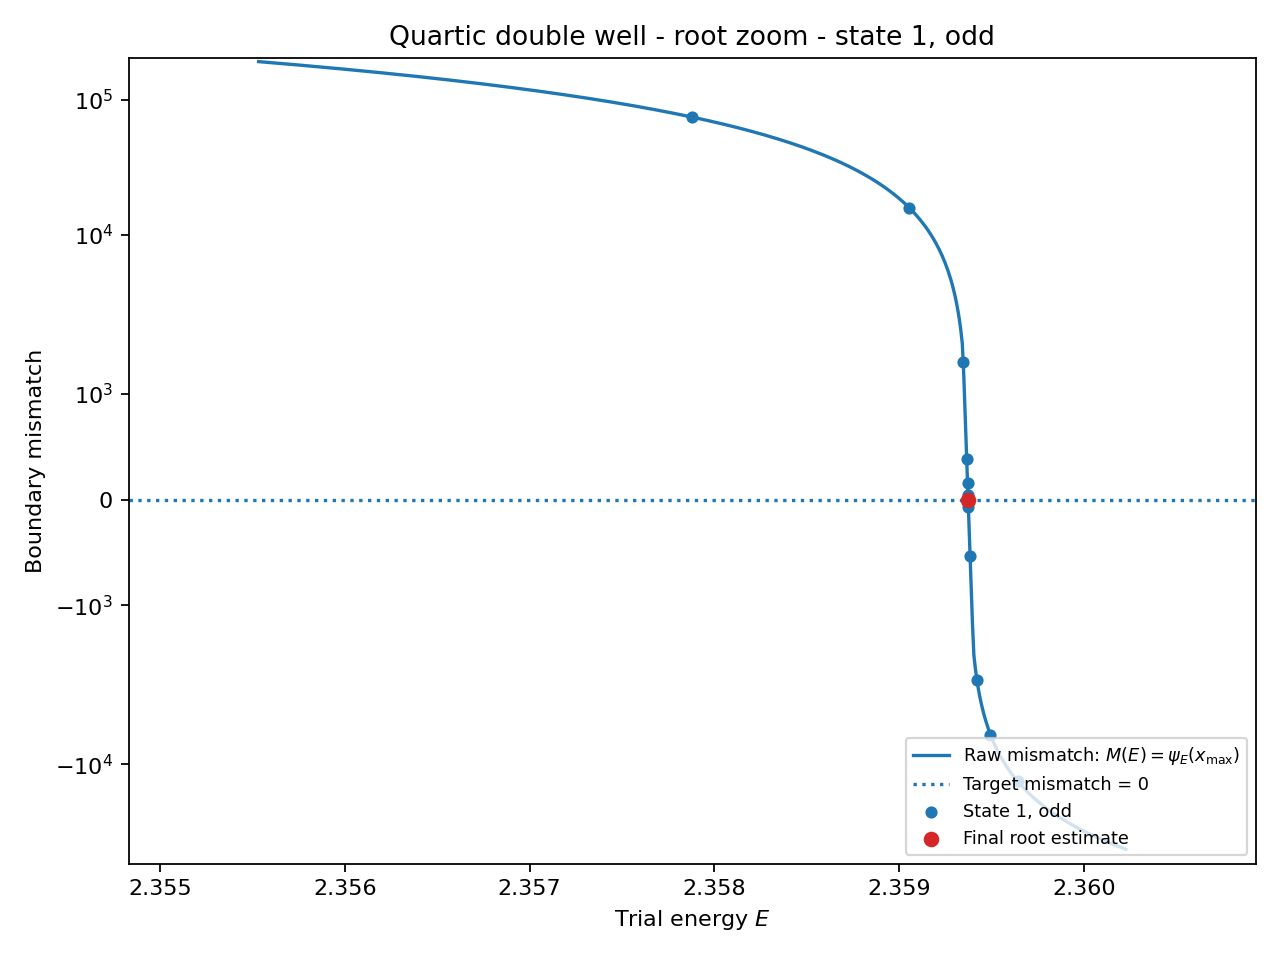
\includegraphics[height=5cm]{../../results/3_double_well_Numerov/3_double_well_Numerov_root_finding_state_1_odd_zoom.png}
                        \caption{}
                    \end{subfigure}

                    \captionof{figure}{Zoomed root brackets for the lowest even (a) and odd (b) double-well states. These local panels show the raw mismatch and the recorded bisection sequence inside the initial sign-changing brackets.}
                    \label{fig:dw_shooting_zoom}
                \end{minipage}
            \end{figure}

            \begin{figure}[p]
                \centering

                \begin{minipage}[t]{0.48\textwidth}
                    \centering
                    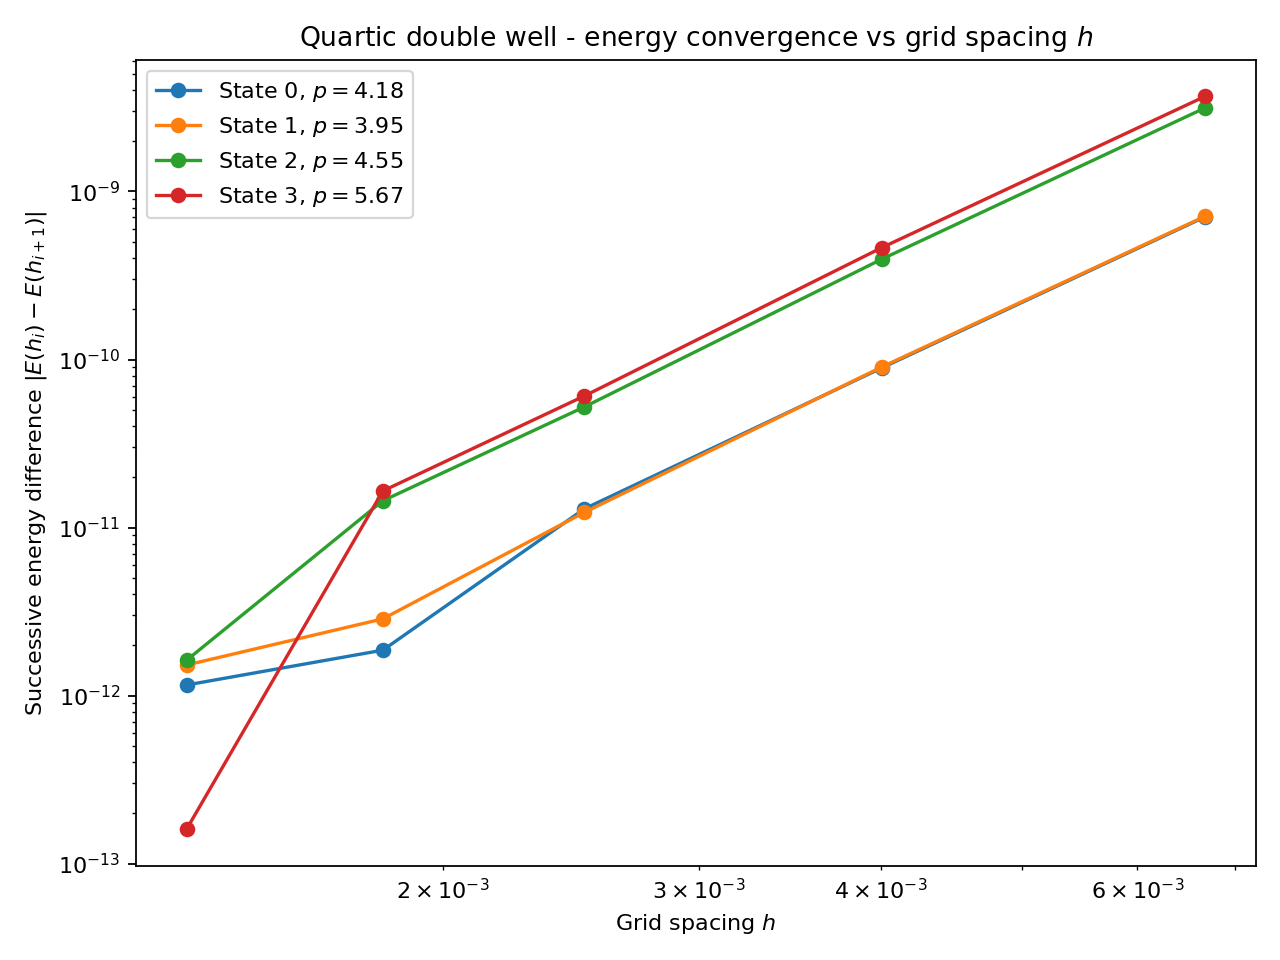
\includegraphics[width=\textwidth]{../../results/3_double_well_Numerov/3_double_well_Numerov_energy_convergence_vs_h.png}
                    \captionof{figure}{Grid convergence for the quartic double well. The energy errors decrease with high-order behavior under successive grid refinement.}
                    \label{fig:dw_convergence_h}
                \end{minipage}
                \hfill
                \begin{minipage}[t]{0.48\textwidth}
                    \centering
                    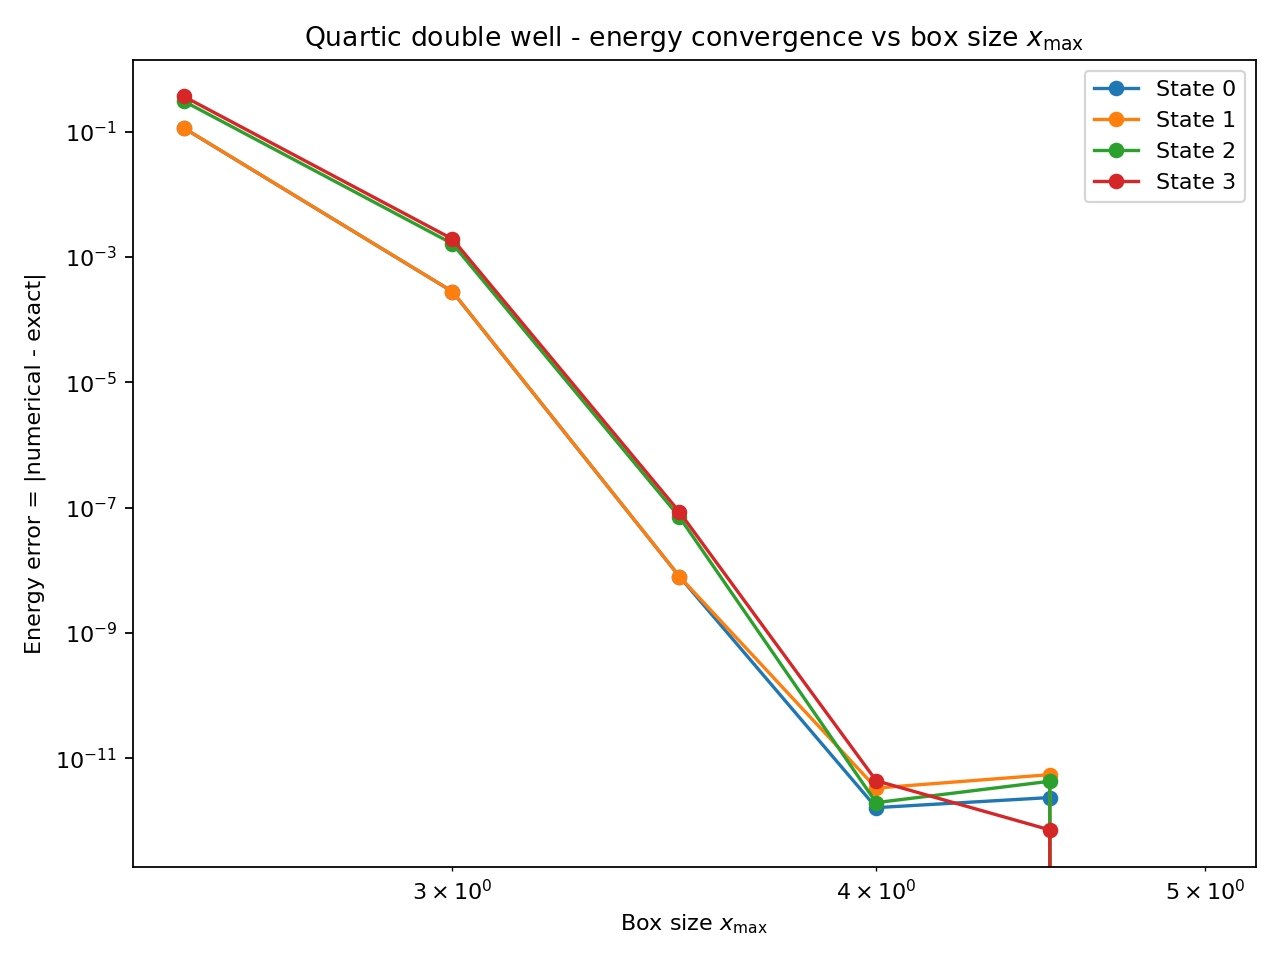
\includegraphics[width=\textwidth]{../../results/3_double_well_Numerov/3_double_well_Numerov_energy_convergence_vs_x_max.png}
                    \captionof{figure}{Dependence of the double-well energy errors on box size. The errors decrease rapidly as the domain is enlarged and then reach a numerical plateau.}
                    \label{fig:dw_convergence_xmax}
                \end{minipage}

                \vspace{1em}

                \begin{minipage}[t]{0.48\textwidth}
                    \centering
                    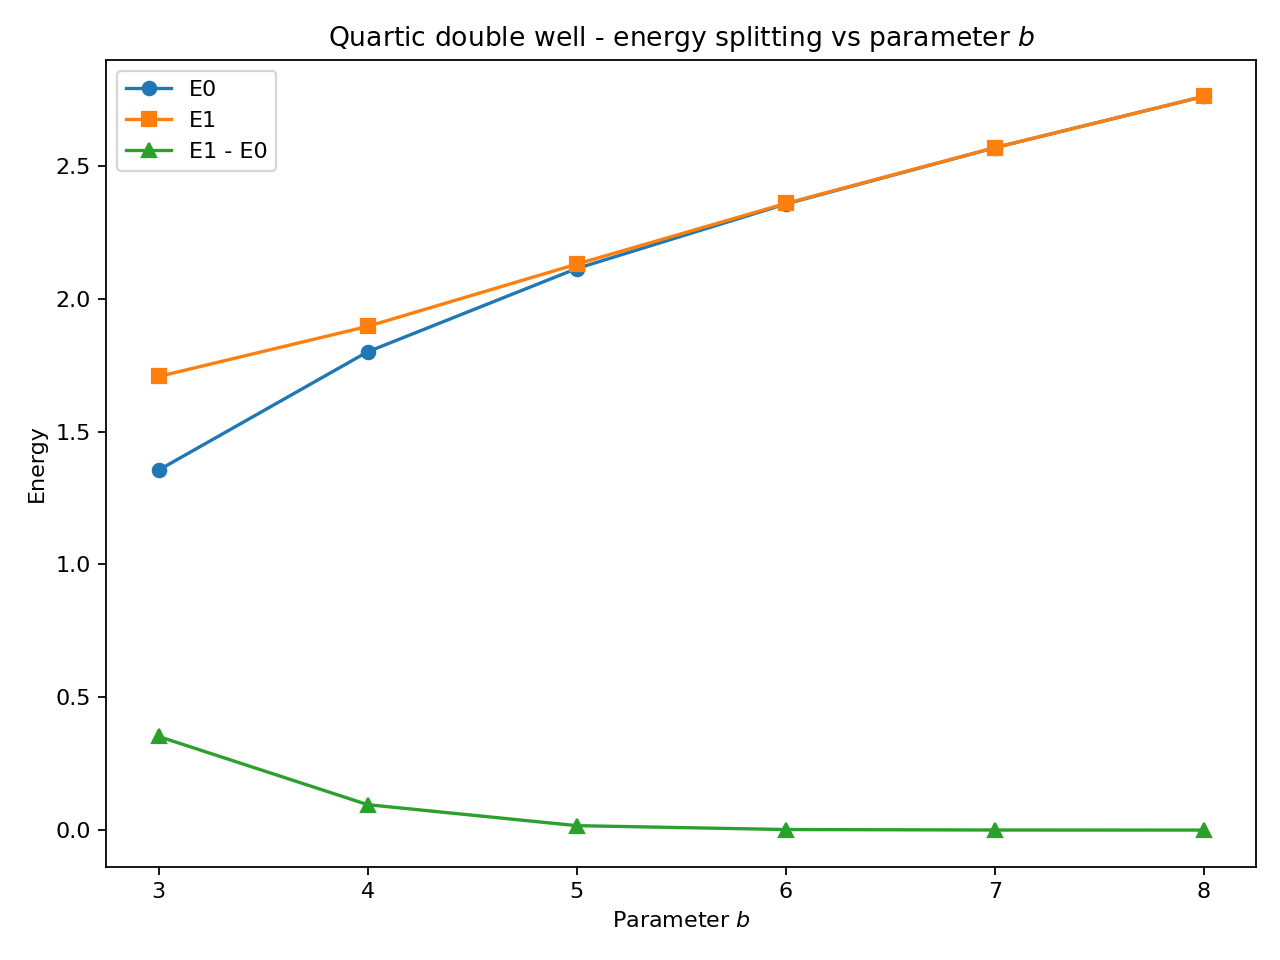
\includegraphics[width=\textwidth]{../../results/3_double_well_Numerov/3_double_well_Numerov_energy_splitting_vs_b.png}
                    \captionof{figure}{Energy splitting between the two lowest double-well states as the parameter $b$ is varied. The splitting decreases as the barrier becomes stronger, consistent with tunneling suppression.}
                    \label{fig:dw_splitting}
                \end{minipage}
            \end{figure}

        \subsection{Finite square well}
            The finite square well is included as an additional nontrivial bound-state test. Unlike the infinite square well, the potential walls are finite, so bound states can leak into the classically forbidden region. The potential used here has the form:
            \begin{equation}
            V(x)=\begin{cases}
            0 & ,|x|\le a\\
            V_0 & ,|x|>a
            \end{cases}
            \end{equation}
            and only states with $E<V_0$ are true bound states. In the production run, the well parameters are $a=1$ and $V_0=12$, while the outward-shooting box uses $x_{\max}=4$ and the Numerov mesh uses $n_{\text{grid}}=3000$. \\

            Figure~\ref{fig:finitewell_states} shows the first four computed states together with the finite well potential. For the parameter choice $V_0=12$ and $a=1$, the four reported bound-state energies are $E_0\approx0.847846$, $E_1\approx3.344466$, $E_2\approx7.294436$, and $E_3\approx11.782210$. The first three lie comfortably below the barrier and are localized mainly inside the well, with exponentially decaying tails outside. The fourth state is only about $0.218$ below the barrier top, so it is a near-threshold bound state and therefore shows much stronger leakage into the exterior region. This is exactly the behavior expected for a finite well, where weaker binding implies a longer evanescent decay length outside the classically allowed region. \\

            The probability densities in Fig.~\ref{fig:finitewell_densities} show the same effect even more clearly. The low-lying states are concentrated inside the well and retain the expected even-odd node ordering, while the highest plotted state has substantial weight outside $|x|\le a$. That long exterior tail is physically correct: unlike the infinite well, a finite barrier does not force the wavefunction to vanish at the walls, it only makes the outside amplitude decay exponentially. \\

            The finite-well root diagnostics in Fig.~\ref{fig:finitewell_shooting} add an important numerical interpretation. In the even-sector global scan, the raw mismatch becomes small again as $E$ approaches the barrier height $V_0=12$ from below. This does not indicate an additional bound state. As $E\to V_0^{-}$, the exterior decay constant $\kappa=\sqrt{2(V_0-E)}$ tends to zero, so on a fixed box the boundary value $\psi_E(x_{\max})$ can decrease in magnitude without actually crossing zero. The zoomed near-threshold brackets in Fig.~\ref{fig:finitewell_shooting_zoom} show the correct interpretation: the reported high-energy roots are genuine sign changes, but the later drift of the raw mismatch toward zero remains one-sided and therefore does not create more bound states. Since true bound states require $E<V_0$, extending the scan to $E>V_0$ would enter continuum behavior rather than reveal extra discrete levels. \\

            These results are sufficient for the finite square well part of the report because this case is used mainly to demonstrate that the same shooting framework works for a potential with finite barriers and evanescent tails. The more detailed convergence and validation analysis is already provided by the infinite well and harmonic oscillator, while the finite well serves as an additional qualitative and physical test. In particular, the finite-well figures confirm that the solver distinguishes strongly bound interior states from a near-threshold state with pronounced barrier penetration. \\

            \begin{figure}[p]
                \centering

                \begin{minipage}[t]{0.48\textwidth}
                    \centering
                    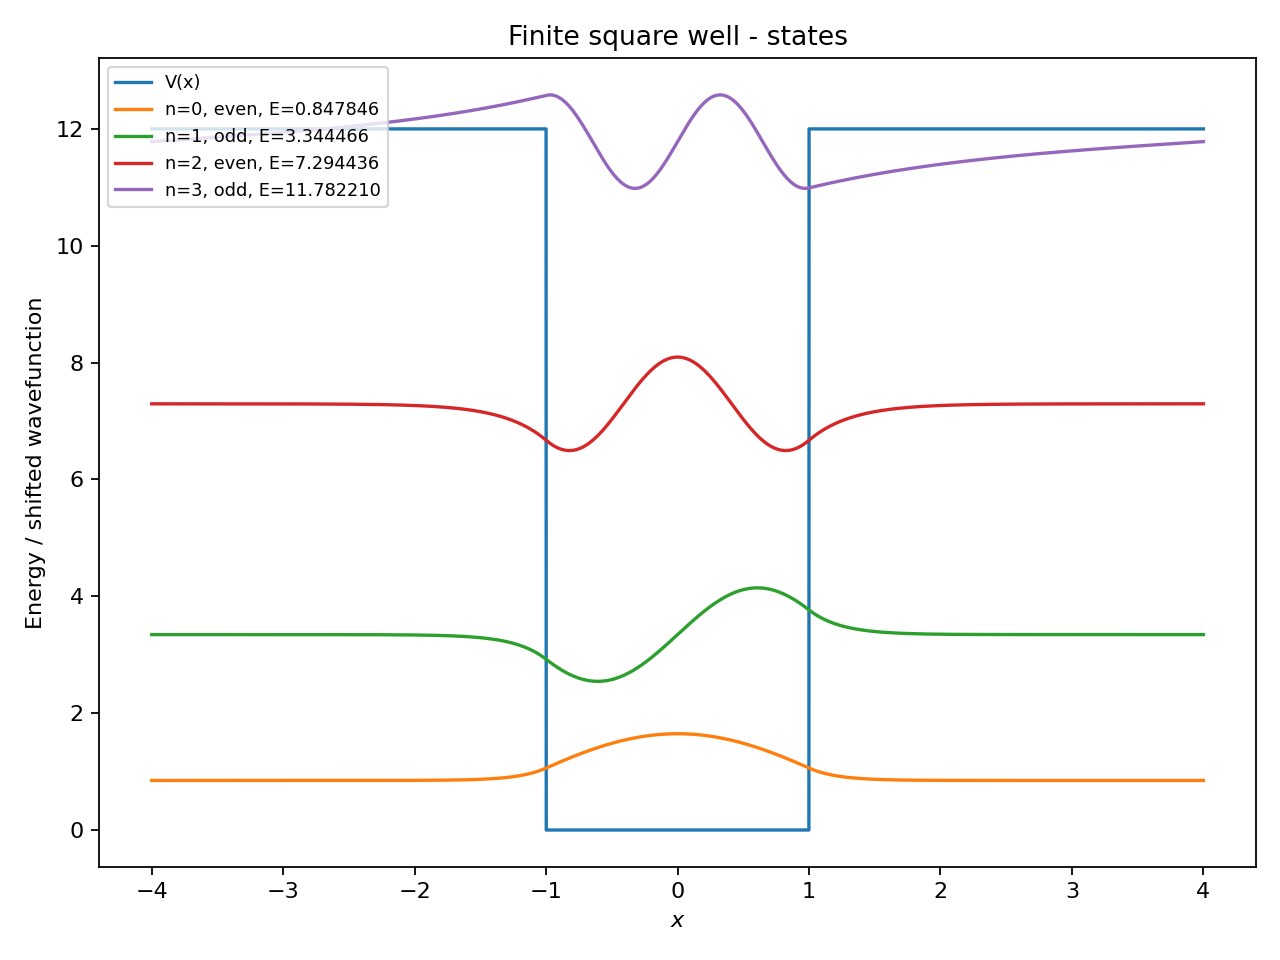
\includegraphics[width=\textwidth]{../../results/4_finite_square_well_Numerov/4_finite_square_well_Numerov_states.png}
                    \captionof{figure}{First four finite square well states plotted together with the finite barrier potential. States below the barrier are localized in the well, while the near-threshold state has a larger evanescent tail.}
                    \label{fig:finitewell_states}
                \end{minipage}
                \hfill
                \begin{minipage}[t]{0.48\textwidth}
                    \centering
                    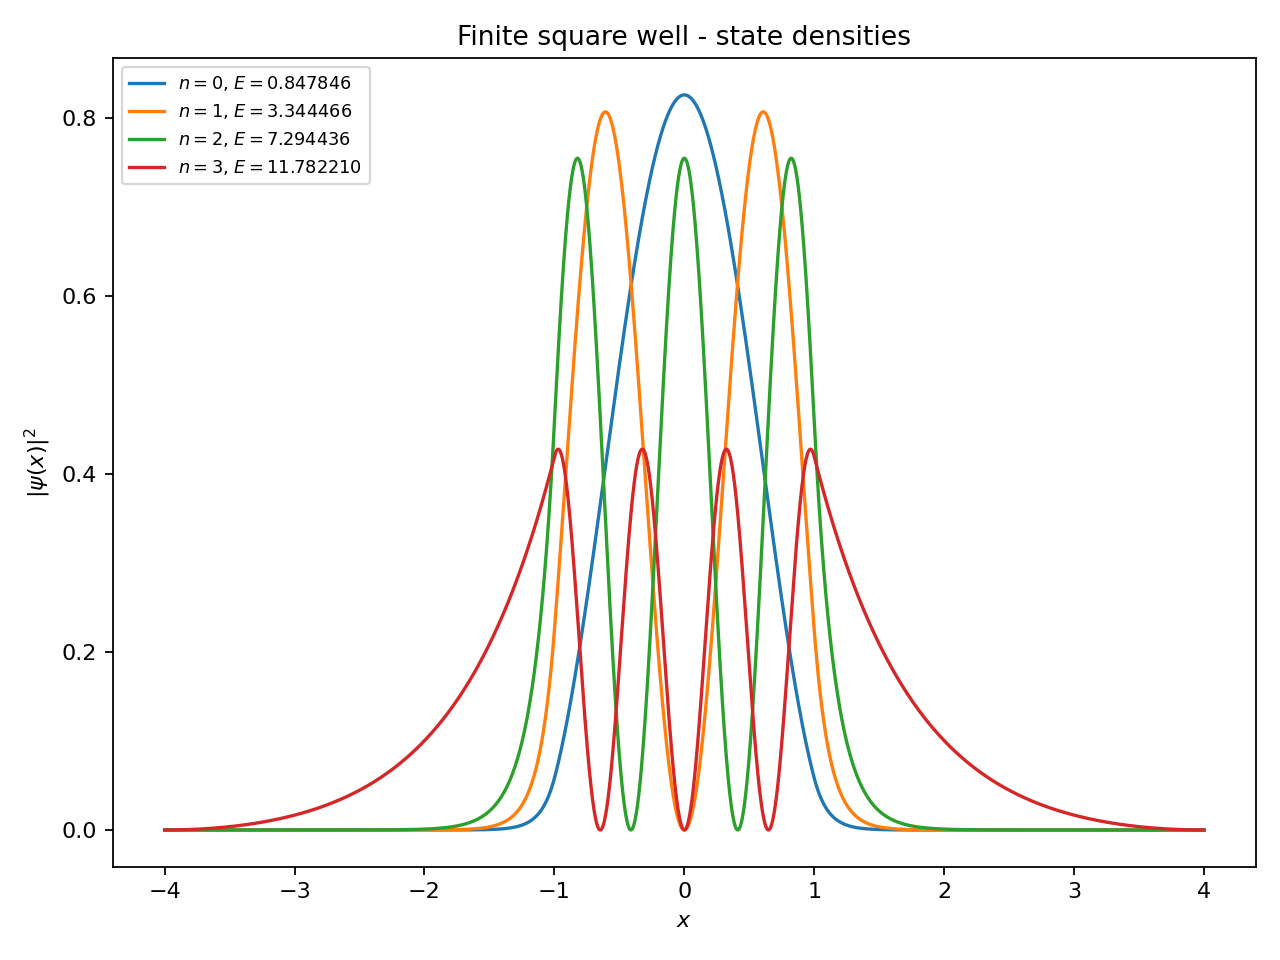
\includegraphics[width=\textwidth]{../../results/4_finite_square_well_Numerov/4_finite_square_well_Numerov_state_densities.png}
                    \captionof{figure}{Probability densities $|\psi(x)|^2$ for the first four finite square well states. The densities show both interior oscillation and exterior exponential leakage.}
                    \label{fig:finitewell_densities}
                \end{minipage}

                \vspace{1em}

                \begin{minipage}[t]{\textwidth}
                    \centering
                    \begin{subfigure}[t]{0.485\textwidth}
                        \centering
                        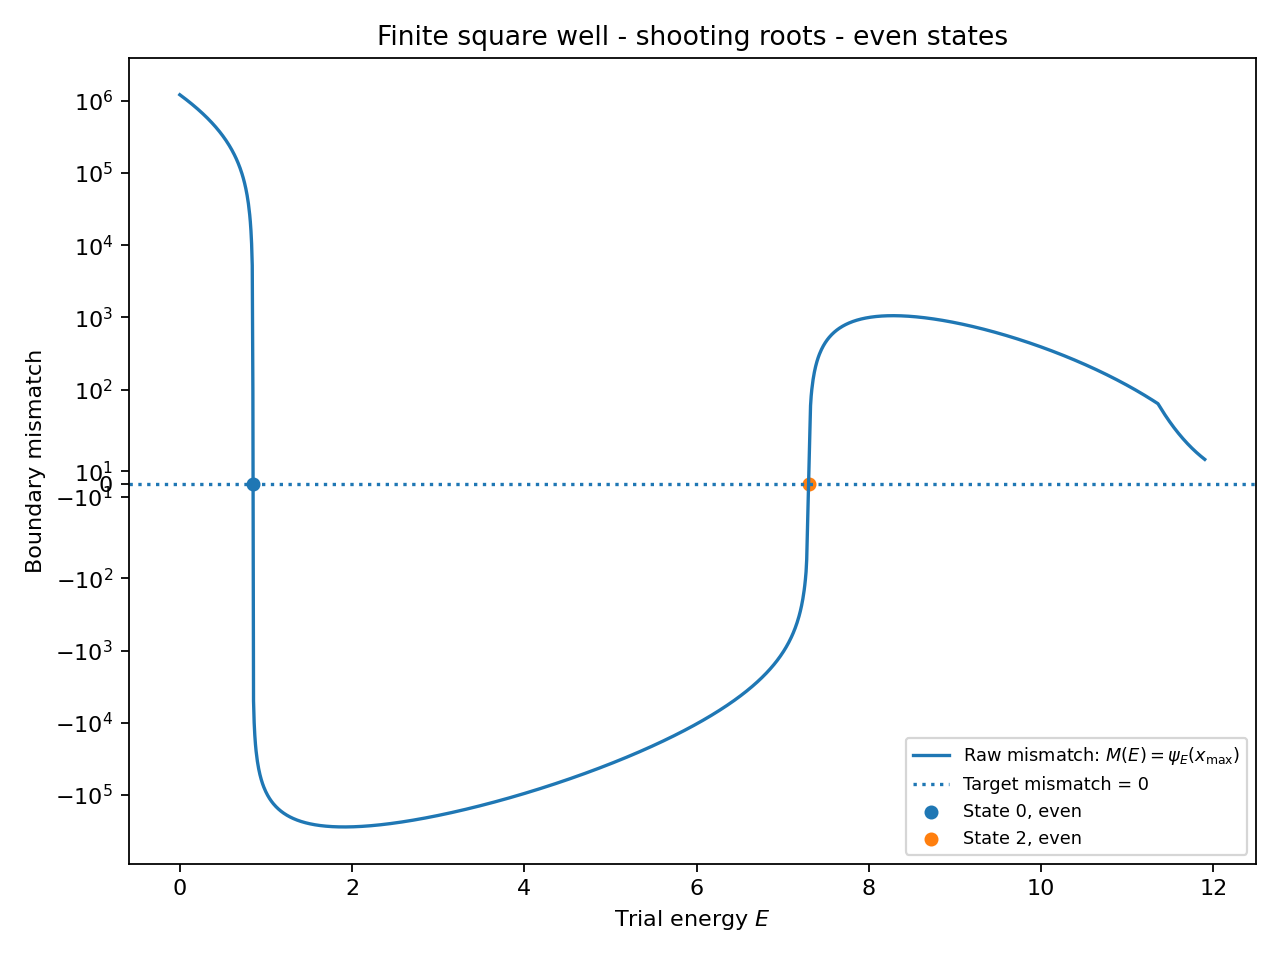
\includegraphics[height=5cm]{../../results/4_finite_square_well_Numerov/4_finite_square_well_Numerov_root_finding_even.png}
                        \caption{}
                    \end{subfigure}
                    \hfill
                    \begin{subfigure}[t]{0.485\textwidth}
                        \centering
                        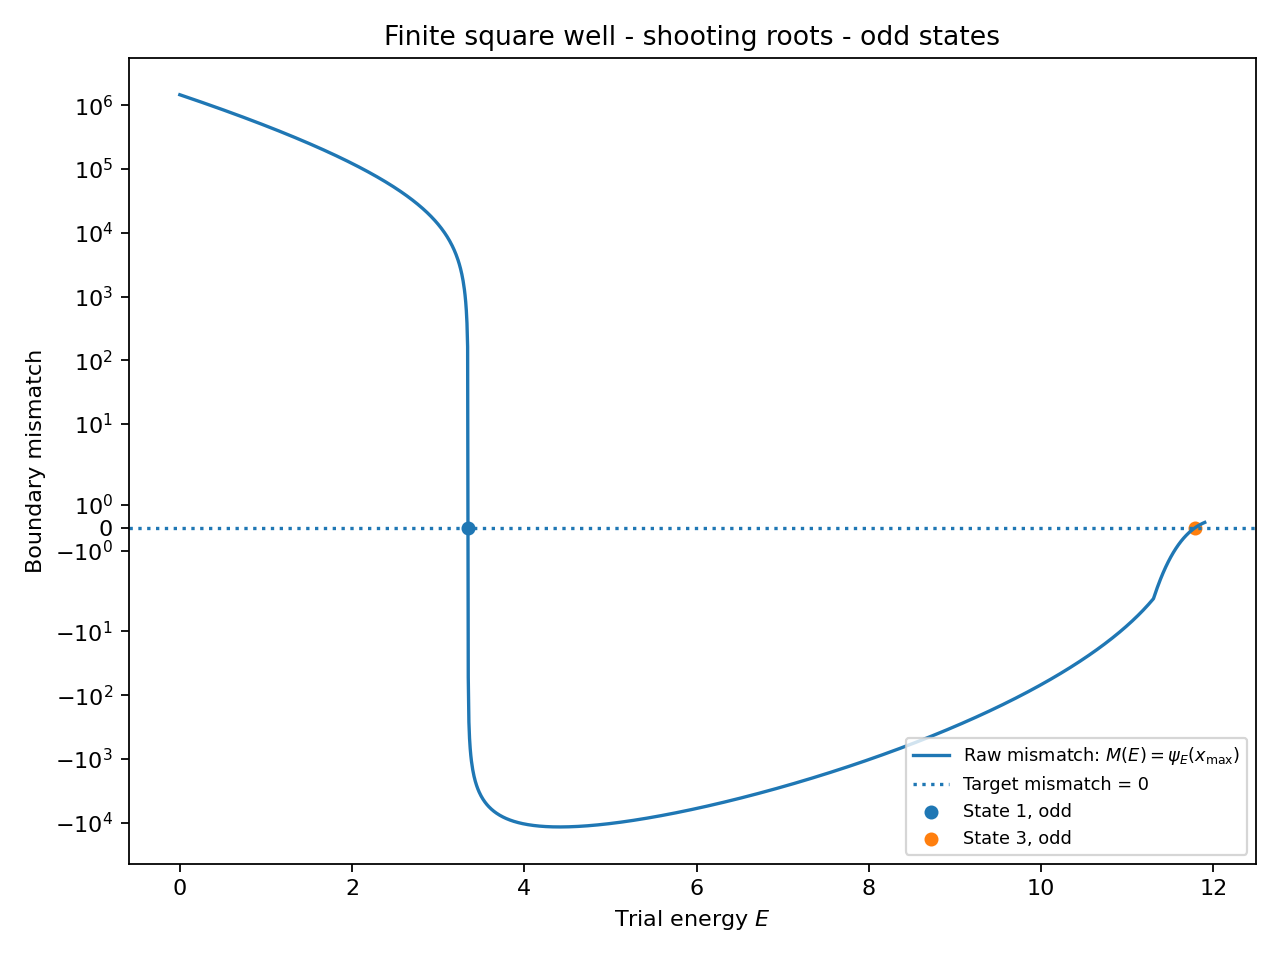
\includegraphics[height=5cm]{../../results/4_finite_square_well_Numerov/4_finite_square_well_Numerov_root_finding_odd.png}
                        \caption{}
                    \end{subfigure}

                    \captionof{figure}{Raw shooting mismatch functions for even (a) and odd (b) finite-well states. The global scans include the near-threshold regime just below the barrier top $V_0$.}
                    \label{fig:finitewell_shooting}
                \end{minipage}

                \vspace{1em}

                \begin{minipage}[t]{\textwidth}
                    \centering
                    \begin{subfigure}[t]{0.485\textwidth}
                        \centering
                        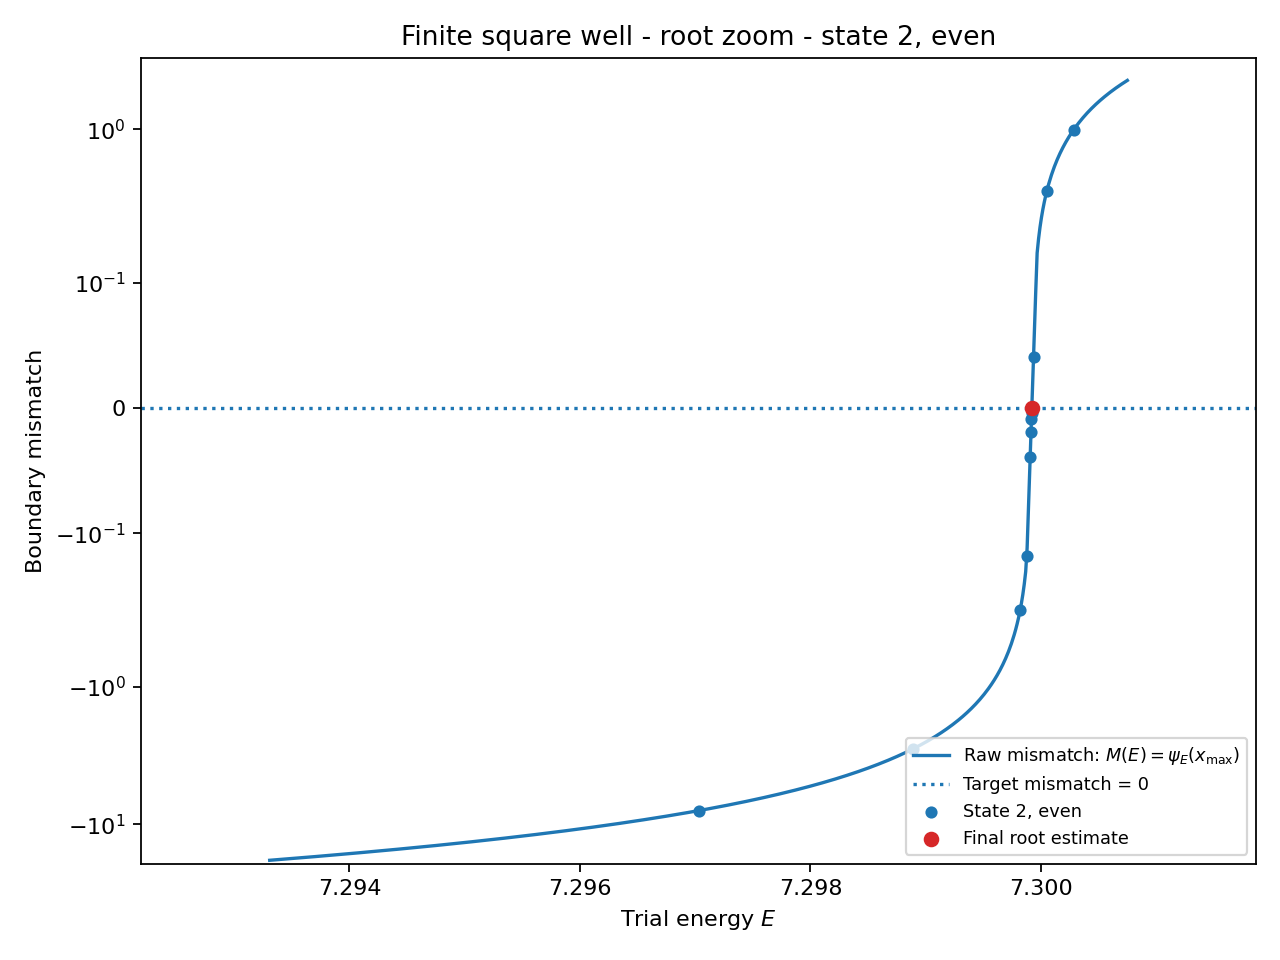
\includegraphics[height=5cm]{../../results/4_finite_square_well_Numerov/4_finite_square_well_Numerov_root_finding_state_2_even_zoom.png}
                        \caption{}
                    \end{subfigure}
                    \hfill
                    \begin{subfigure}[t]{0.485\textwidth}
                        \centering
                        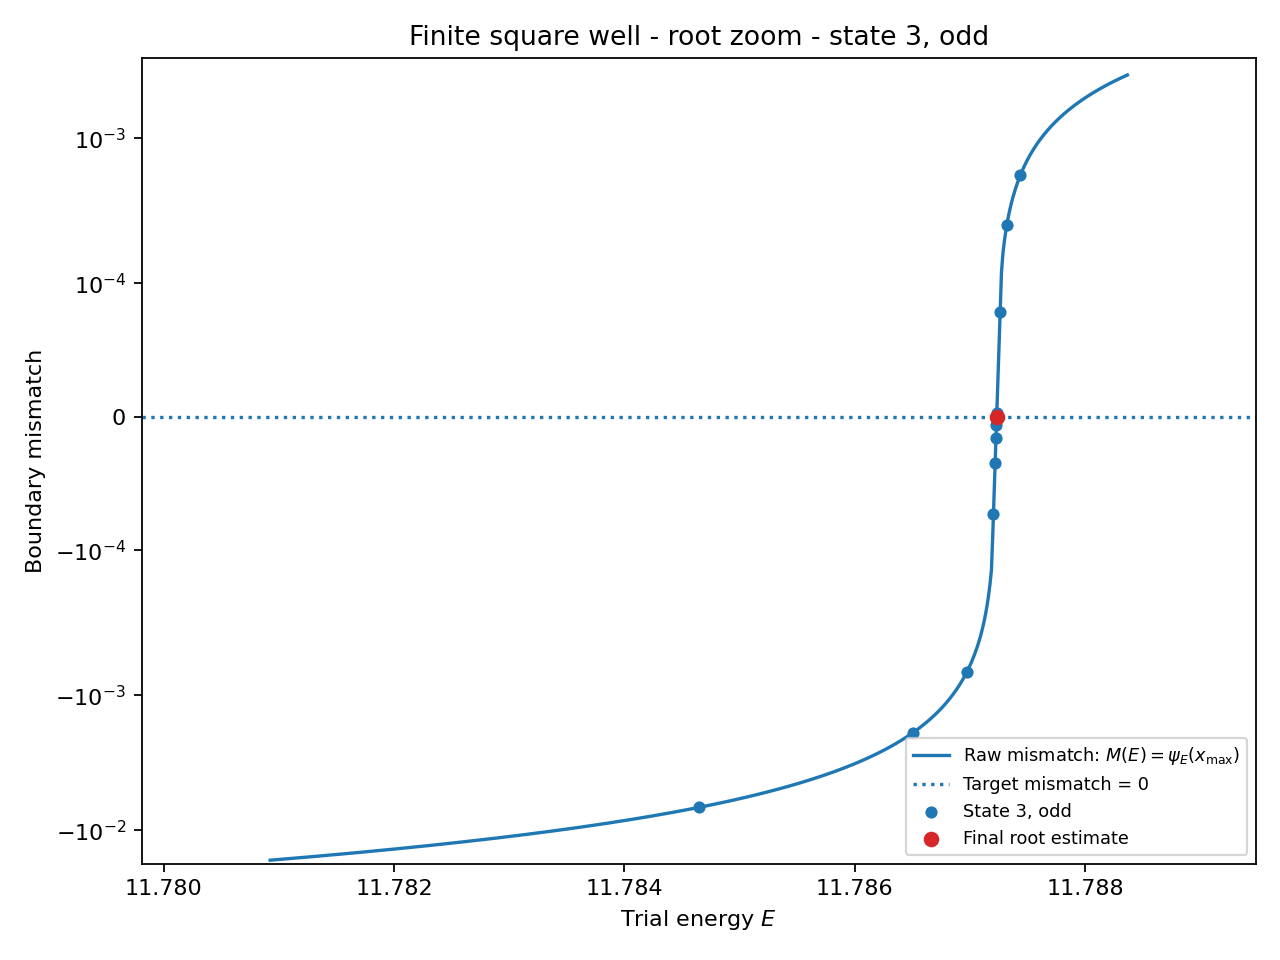
\includegraphics[height=5cm]{../../results/4_finite_square_well_Numerov/4_finite_square_well_Numerov_root_finding_state_3_odd_zoom.png}
                        \caption{}
                    \end{subfigure}

                    \captionof{figure}{Zoomed near-threshold brackets for the higher even (a) and odd (b) finite-well bound states. These views isolate the genuine sign-changing roots close to the barrier top and show the full recorded bisection history.}
                    \label{fig:finitewell_shooting_zoom}
                \end{minipage}
            \end{figure}

        \subsection{Scattering and resonant tunneling}
            \subsubsection{Single barrier potential}
                As a secondary extension beyond bound states, the Numerov framework is also applied to one-dimensional scattering from a finite rectangular barrier. For each incident energy $E$, the complex wavefunction is propagated through the barrier region and decomposed into incident, reflected, and transmitted waves. This gives the transmission and reflection probabilities $T(E)$ and $R(E)$. \\

                The shared scattering grid for both barrier problems is $x\in[-8,8]$ with $n_{\text{grid}}=4000$ points. For the single-barrier run, the barrier parameters are $V_0=5$, width $1.2$, and center $0$, while the incident energy is sampled on $240$ points from $E=0.2$ to $E=10$. \\

                The single-barrier result is shown in Fig.~\ref{fig:single_barrier_scattering}. For the saved run the barrier has height $V_0=5$ and width $1.2$, while the incident energy is scanned from $0.2$ to $10$. At low incident energy, where $E$ is well below the barrier height, transmission is strongly suppressed and reflection is close to one; for example, at $E=0.2$ the calculation gives $T\approx3.6\times10^{-4}$ and $R\approx0.99964$. As the incident energy increases through and above the barrier, transmission rises and reflection falls, which is the expected qualitative behavior for a finite barrier. \\

                The curve also shows an important physical detail: even for $E>V_0$, transmission is not exactly one. The barrier still causes partial reflection because the wave number changes across the interfaces. In the saved data, $T(E)$ reaches its maximum value very close to one near $E\approx8.4$, but by $E=10$ it is still only about $0.956$, with a residual reflection of about $0.044$. That is fully consistent with above-barrier scattering from a finite rectangular barrier rather than a sharp classical step from total reflection to total transmission. \\

                The dashed curve shows the conservation check $T(E)+R(E)$, which is numerically indistinguishable from one across the full energy range in the saved data: the largest deviation is about $2.3\times10^{-12}$. This confirms that the numerical scattering calculation conserves probability flux to within floating-point error for this setup. \\

                \begin{figure}[h]
                    \centering
                    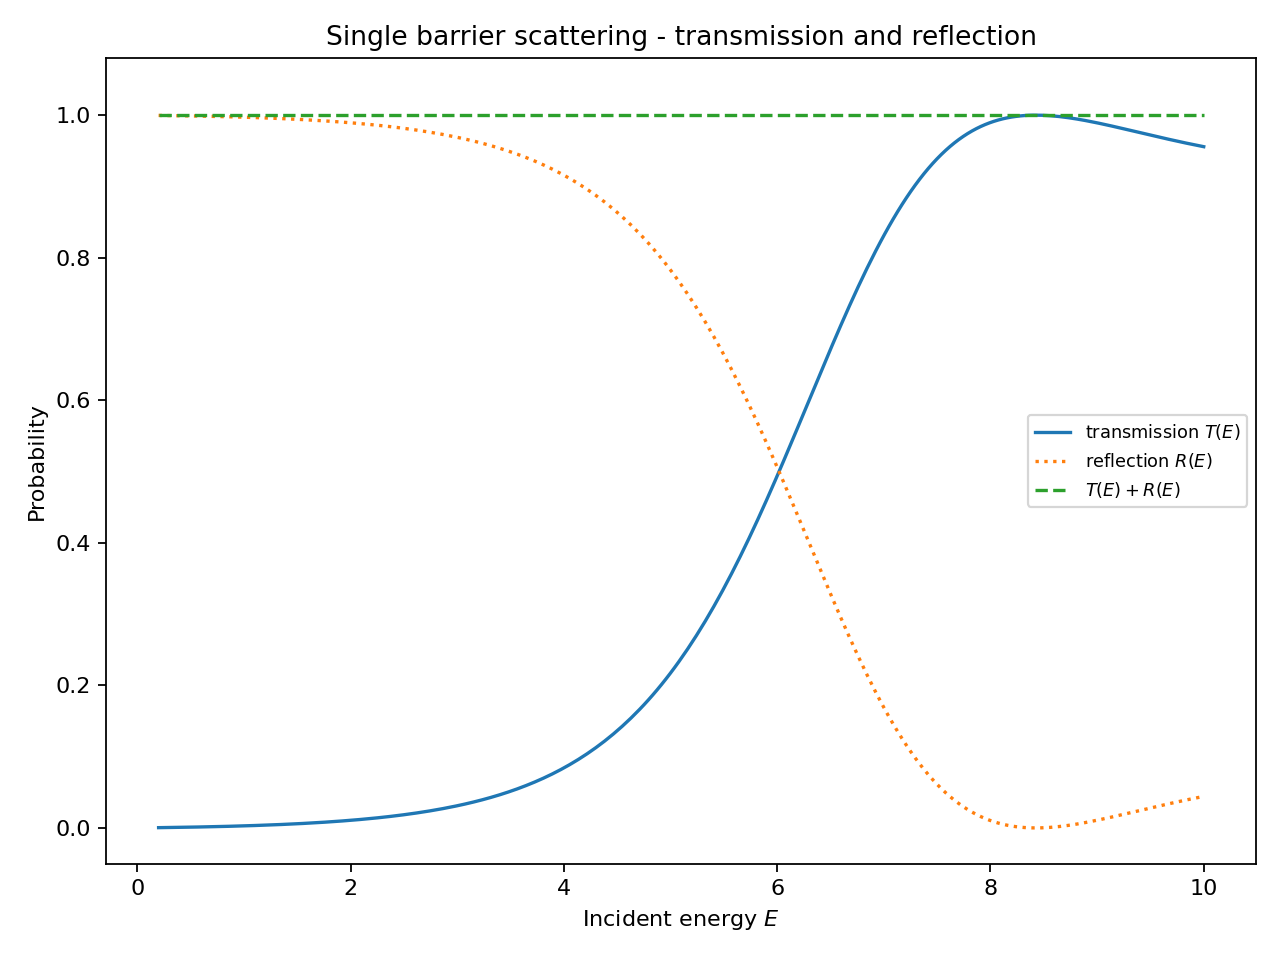
\includegraphics[height=5cm]{../../results/5_scattering_single_barrier_Numerov/5_scattering_single_barrier_Numerov_transmission_reflection.png}
                    \caption{Transmission and reflection probabilities for scattering from a finite rectangular barrier. At low energies reflection dominates, while at high energies transmission approaches unity. The conservation check $T(E)+R(E)$ remains close to one.}
                    \label{fig:single_barrier_scattering}
                \end{figure}

            \subsubsection{Double barrier potential}
                The double-barrier potential is used to demonstrate resonant tunneling. In this case the two barriers create an intermediate well, so certain incident energies can form quasi-bound states between the barriers. At these energies, destructive reflection and constructive transmission lead to sharp peaks in the transmission coefficient. \\

                For the production double-barrier run, each barrier has height $V_0=5$, the barrier width is $0.6$, the central well width is $1.4$, the structure is centered at $x=0$, and the incident energy is sampled on $420$ points from $E=0.2$ to $E=5.0$. Resonance candidates are then identified from the transmission curve using a simple peak threshold of $T(E)>0.65$. \\

                Figure~\ref{fig:double_barrier_resonances} shows the computed transmission and reflection probabilities for two barriers separated by a central well. The saved transmission curve contains two clear resonances: a very narrow low-energy peak at $E\approx1.13938$ with $T\approx0.99996$, and a broader high-energy peak at $E\approx4.35847$ with $T\approx0.99987$. At both resonant energies, reflection is almost completely suppressed. This is the expected behavior for resonant tunneling: when the incident energy matches a quasi-bound mode of the region between the barriers, multiple reflections inside the central well interfere constructively for transmission and destructively for reflection. \\

                The conservation check $T(E)+R(E)$ is again essentially exact in the saved calculation, with a largest deviation of about $8.4\times10^{-12}$. This is an important diagnostic because it verifies that the numerical decomposition into incident, reflected, and transmitted components is self-consistent over the full energy scan, including very sharp resonances. \\

                The two resonances also have visibly different widths, which is physically meaningful. The first peak is extremely narrow, indicating a longer-lived quasi-bound state with weaker leakage through the barriers, while the second peak is much broader, indicating stronger coupling to the external scattering channels. That broader width is why the transmission stays elevated over a larger energy interval around the second resonance. \\

                Figure~\ref{fig:double_barrier_resonant_state} shows the probability density at the first resonance. The wavefunction is strongly enhanced in the region between the two barriers, with only much smaller amplitude outside. This is the expected signature of a quasi-bound state trapped temporarily in the central well, and it explains the near-unit transmission at the corresponding resonant energy. \\

                These results are sufficient for the double-barrier part of the report because the scattering section is a secondary extension. The plots demonstrate the key qualitative physics: transmission resonances, reflection suppression at resonance, flux conservation, and resonant enhancement of the wavefunction in the central well. \\

                \noindent
                \begin{minipage}[t]{0.48\textwidth}
                    \centering
                    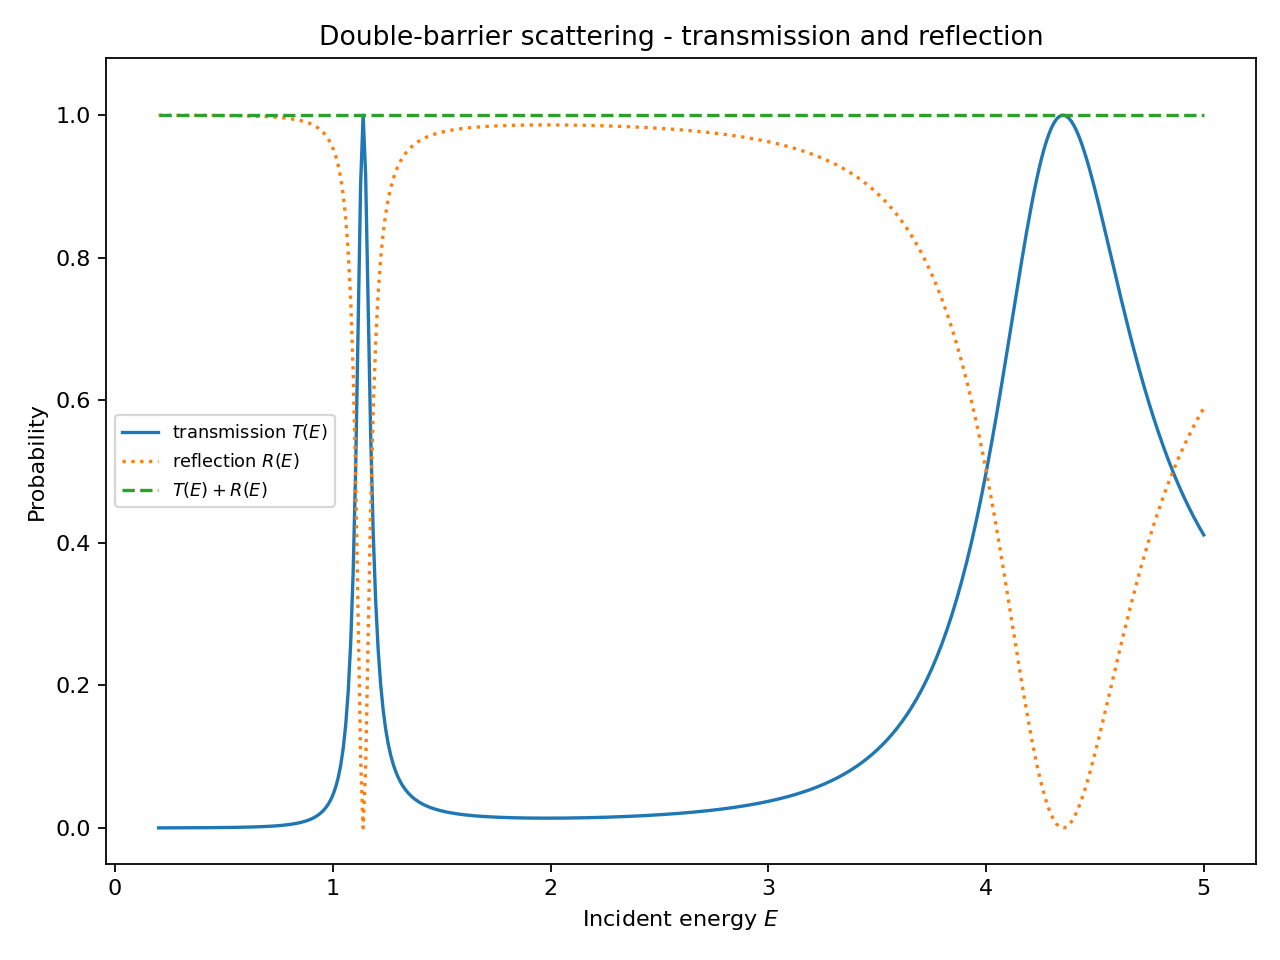
\includegraphics[width=\textwidth]{../../results/6_scattering_double_barrier_Numerov/6_scattering_double_barrier_Numerov_transmission_reflection.png}
                    \captionof{figure}{Transmission and reflection probabilities for the double-barrier potential. Sharp transmission peaks occur at resonant energies, where reflection is suppressed and $T(E)+R(E)$ remains close to one.}
                    \label{fig:double_barrier_resonances}
                \end{minipage}
                \hfill
                \begin{minipage}[t]{0.48\textwidth}
                    \centering
                    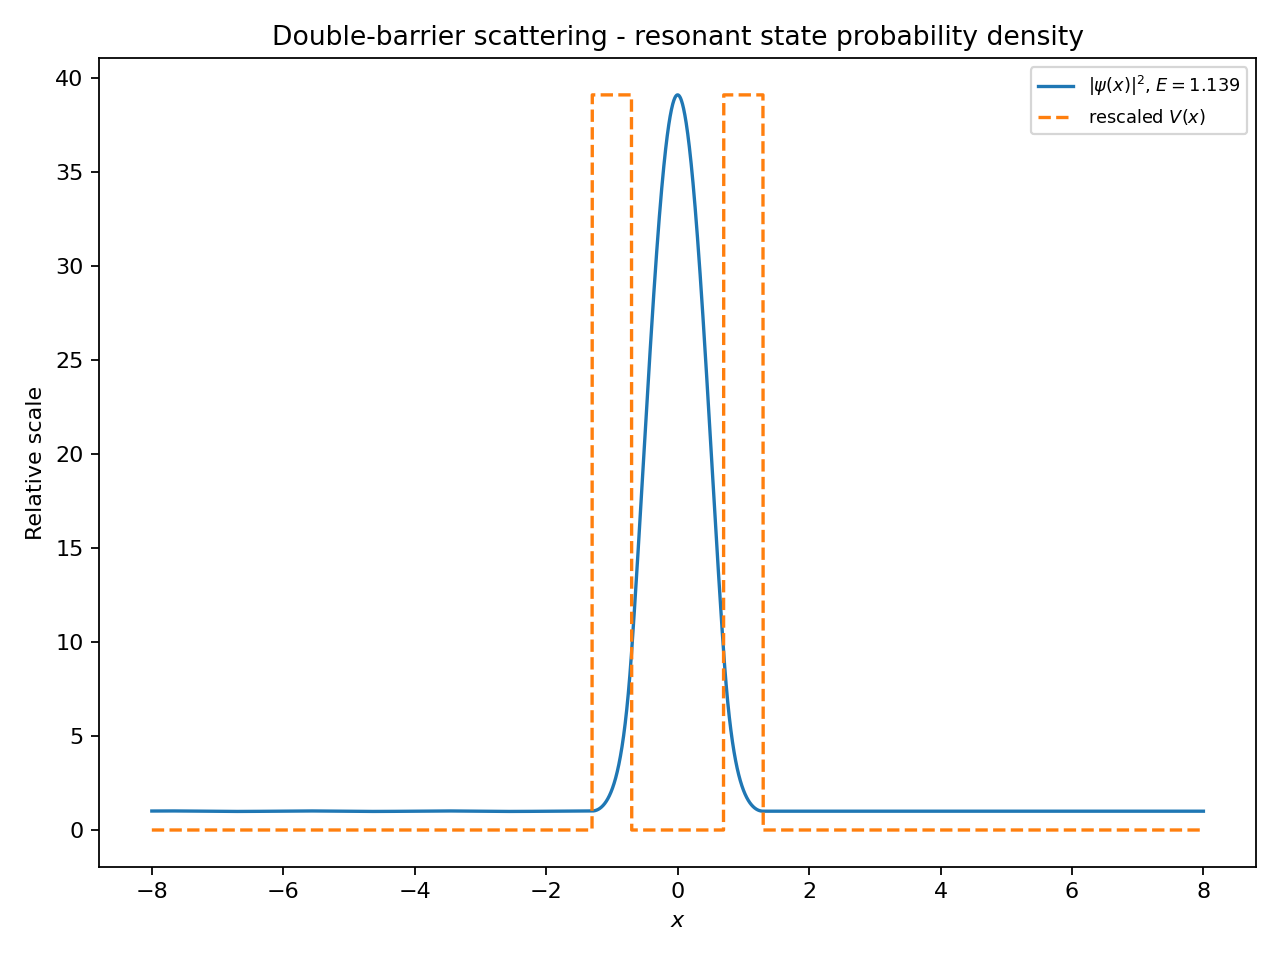
\includegraphics[width=\textwidth]{../../results/6_scattering_double_barrier_Numerov/6_scattering_double_barrier_Numerov_state_probability_density.png}
                    \captionof{figure}{Probability density at the first resonant energy. The wavefunction is strongly enhanced between the two barriers, showing the quasi-bound state responsible for resonant tunneling.}
                    \label{fig:double_barrier_resonant_state}
                \end{minipage}

    % ==============================================================
    % Discussion
    % ==============================================================
    \section{Discussion}
        The calculation was checked in four complementary ways. First, an automated validation suite tests normalization, the fourth-order boundary derivative, analytic benchmark energies, the double-well level ordering, scattering flux conservation, and the entry-script import path. Second, the infinite square well and harmonic oscillator reproduce known analytic spectra, providing direct validation of the eigenvalue search. In the saved runs, the first four square-well relative errors are of order $10^{-11}$--$10^{-10}$, and the first four harmonic-oscillator relative errors are of order $10^{-12}$--$10^{-11}$. Third, the wavefunctions have the expected parity, node structure, normalization, and boundary behavior. Fourth, convergence tests with respect to grid spacing and domain size show that the results are stable under numerical refinement. \\

        The convergence behavior also exposes important numerical details. In the infinite square well, the observed fourth-order convergence confirms that the Numerov recurrence, startup conditions, and boundary treatment are consistent. For the harmonic oscillator, the box-size study separates domain truncation error from discretization error: increasing $x_{\max}$ initially reduces the error rapidly, after which the error reaches a plateau set by grid spacing, root-finding tolerance, and floating-point limits. Slopes slightly above fourth order in some fits are therefore interpreted as small-error fitting artifacts rather than evidence of a truly higher-order method. The same caution applies in the double-well case, where successive-refinement fits above fourth order appear only once the differences are already near the numerical floor. \\

        The comparison with RK4 shows why method order alone is not enough. RK4 evolves both $\psi$ and $\psi'$ directly, while Numerov requires numerical boundary diagnostics. Once the boundary derivative in the Numerov inward-shooting calculation is evaluated with comparable accuracy, Numerov behaves as expected and gives smaller errors than RK4 at the same grid spacing for the harmonic oscillator, typically by a factor of about $2$--$4$ in the saved max-error comparison. \\

        For the quartic double well, where no closed-form spectrum is available, correctness is established through self-consistency rather than analytic comparison. The use of an analytic potential shift, separated grid and box convergence studies, parity-specific root diagnostics, and normalized boundary leakage all support the reliability of the computed states. The low-lying even-odd pair at $b=6$ has the expected small tunneling splitting, about $2.10\times10^{-3}$, and the splitting decreases systematically to about $1.59\times10^{-5}$ by $b=8$, which is the expected physical signature of tunneling suppression. \\

        The finite square well provides an intermediate physical check between analytic bound-state benchmarks and more complex tunneling problems. Its low-lying states remain localized inside the well, while the highest bound state lies only about $0.218$ below the barrier and therefore shows the expected long evanescent tail outside the well. This confirms that the same shooting framework handles both hard-wall-like confinement and finite barrier penetration. \\

        The scattering examples are treated as a secondary extension. The single-barrier calculation shows the expected transition from reflection-dominated behavior at low energy to transmission-dominated behavior at high energy, while still retaining nonzero above-barrier reflection from interface mismatch. The double-barrier calculation shows two resonant transmission peaks, near $E\approx1.13938$ and $E\approx4.35847$, together with strong probability-density enhancement in the central well at resonance. In both cases, the saved calculations satisfy $T(E)+R(E)=1$ to within about $10^{-11}$--$10^{-12}$, providing an additional numerical consistency check. \\

    % ==============================================================
    % Conclusion
    % ==============================================================
    \section{Conclusion}
        This project implemented a Numerov shooting solver for the one-dimensional time-independent Schr\"odinger equation. The method was validated on analytic bound-state problems, extended to finite and double-well potentials, and checked through convergence studies, parity diagnostics, and comparison with RK4. \\

        The benchmark results are quantitatively strong. The infinite square well and harmonic oscillator reproduce the expected spectra to very high precision, with fourth-order convergence recovered once boundary conditions and startup terms are treated consistently. The harmonic-oscillator comparison also shows that the specialized Numerov scheme achieves smaller errors than RK4 at the same grid spacing when both are implemented carefully. \\

        Beyond the analytic tests, the finite square well and quartic double well show the expected physical behavior: barrier penetration in the finite well, a near-degenerate tunneling doublet in the double well, and a splitting that decreases rapidly as the wells are deepened and separated. The scattering extension further reproduces the expected transition from ordinary tunneling through a single barrier to resonant transmission through a double barrier, with probability flux conserved to near machine precision throughout. \\

        Overall, the results support the main conclusion of the project: Numerov shooting is an accurate and flexible method for one-dimensional quantum bound-state and scattering calculations, provided that boundary diagnostics, box size, and convergence checks are treated as part of the numerical method rather than as afterthoughts.

    % ==============================================================
    % References
    % ==============================================================
    \printbibliography[heading=bibintoc,title={References}]
    \end{refsection}
\end{document}
